\chapter{Codifica} \label{codifica}

Questo capitolo tratta gli aspetti più interessanti della codifica dell'applicazione \textit{moviORDER}. In particolare, il capitolo è stato diviso in sezioni che trattano la codifica di:
\begin{enumerate}
	\item \textbf{servizio web};
	\item \textbf{logica applicativa};
	\item \textbf{interfaccia grafica}.
\end{enumerate}

\section{Servizio web} \label{codificaservizio}

Per lo sviluppo del servizio web che permette all'applicazione di accedere al \textit{database} presente sul \textit{server cloud} di \visione{} si è utilizzato il linguaggio \textit{Java} e, nello specifico, gli oggetti \textit{servlet}. Per permettere agli oggetti \textit{servlet} di interagire con il \textit{database} si sono dovuti utilizzare i driver \textit{JDBC} per \textit{SQL Server}, in quanto \textit{moviORDER} è basata su tale \textit{database}. 

\subsection{Servlet}

In questa sezione viene presentato l'utilizzo degli oggetti \textit{servlet} nella realizzazione del servizio web. Le classi che implementano gli oggetti \textit{servlet} appartengono al \textit{package} \textit{servlet}.

\subsubsection{Struttura di un oggetto servlet}

Un oggetto \textit{servlet} è una classe \textit{Java} che eredita dalla classe \textit{HttpServlet}, appartenente al \textit{package} \textit{javax.servlet.http}. \textit{HttpServlet} è una classe astratta che può essere estesa per creare un \textit{servlet} \textit{HTTP} utilizzabile per un sito web. Nel progetto realizzato, il servlet è stato utilizzato per acquisire richieste \textit{HTTP POST}, per elaborarle interrogando il \textit{database} sul \textit{server} cloud di \visione{}, e per rispondere ad esse tramite una stringa in formato \textit{JSON}. Ogni \textit{servlet} del servizio web implementa il metodo \textit{protected void doPost(HttpServletRequest req, HttpServletResponse resp)}. Tale metodo viene chiamato dal \textit{server} per permettere all'oggetto \textit{servlet} di acquisire una richiesta POST da parte di un \textit{client}. Nel caso del progetto, il \textit{client} è la logica applicativa dell'applicazione \textit{moviORDER} e il \textit{server} è \textit{Apache Tomcat}.

\textit{HttpServletRequest} è la classe \textit{Java} che rappresenta le richieste \textit{HTTP} che possono essere inviate all'oggetto \textit{servlet}. Tramite opportuni metodi è possibile accedere alle informazioni contenute nella specifica richiesta. Tramite il metodo \textit{String getParameter(String name)} è possibile, data una stringa rappresentante un parametro della richiesta \textit{HTTP}, ottenere una stringa contenente il valore associato a tale parametro, oppure il valore \textit{null} se il parametro non esiste.

\textit{HttpServletResponse} è la classe \textit{Java} che rappresenta la risposta dell'oggetto \textit{servlet} alla richiesta del \textit{client}. Tramite opportuni metodi è possibile configurare la risposta:
\begin{itemize}
	\item \textit{void setContentType(String type)}: permette di impostare la tipologia di contenuto della risposta. Nel progetto la risposta è una stringa in formato \textit{JSON}, quindi è stato impostato il content type \textit{application/json};
	\item \textit{PrintWriter getWriter()}: restituisce un oggetto \textit{PrintWriter} che può essere utilizzato per inviare caratteri di testo al \textit{client}. Nel progetto, l'oggetto \textit{PrintWriter} è stato utilizzato per inviare la stringa di risposta in formato \textit{JSON}.
\end{itemize}

Viene di seguito fornita, a titolo d'esempio, l'implementazione del metodo \textit{doPost()} del \textit{servlet} del servizio web che si occupa di controllare che le credenziali inserite dall'utente in fase di login siano corrette. Nella prossima sezione viene fornito un esempio di come la logica applicativa di \textit{moviORDER} effettua una richiesta a tale \textit{servlet} e di come utilizza la risposta per modificare lo stato dell'applicazione. Nell'esempio, la classe \textit{DatabaseConnection} fornisce un'interfaccia per l'interrogazione di un \textit{database} \textit{SQL Server}. Una spiegazione di tale classe è presente in sezione \ref{dbconnect}.

\begin{figure}[!h] 
    \centering 
    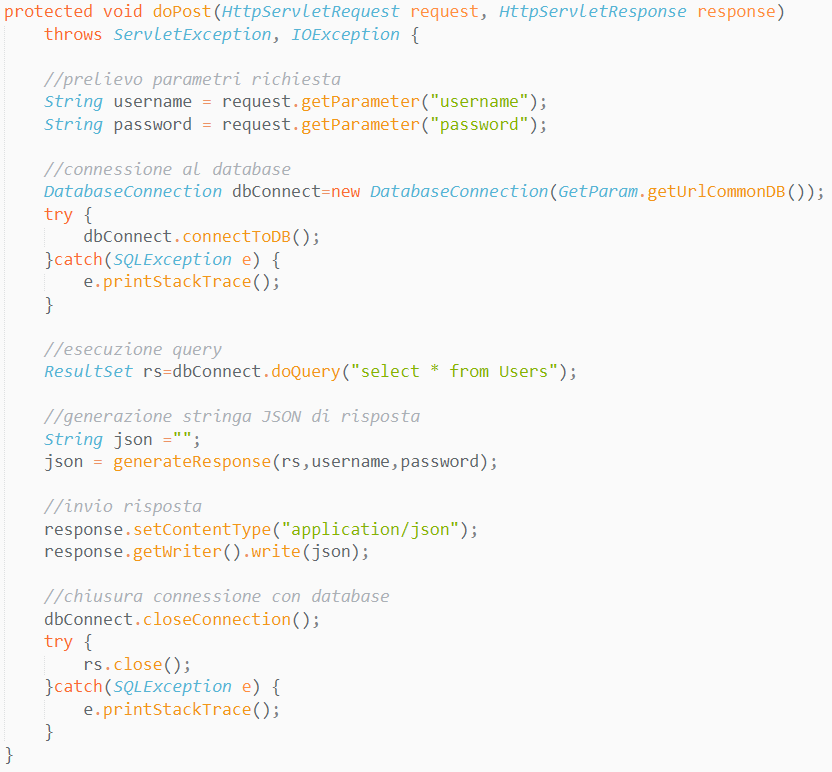
\includegraphics[height=10cm,width=\columnwidth]{codice/servlet} 
    \caption{Metodo \textit{doPost()} del \textit{servlet} che gestisce l'autenticazione}
\end{figure}

\subsubsection{Interrogazione del servizio web}

Nel momento in cui viene implementato un \textit{servlet} concreto, \textit{eclipse} gli associa un \textit{end-point} in automatico. Tramite l'\textit{end-point} è possibile raggiungere il \textit{servlet} sul \textit{server} per effettuare richieste \textit{HTTP}. L'\textit{end-point} associato da \textit{eclipse} è della forma \textit{/NomeClasseServlet} e può essere cambiato dalle impostazioni dell'\textit{IDE}. Per rendere possibile il raggiungimento del servizio web da parte della logica applicativa di \textit{moviORDER}, è necessario che venga effettuato il \textit{deploy} del servizio su \textit{Apache Tomcat} e che quest'ultimo venga fatto girare sul \textit{server cloud} di \visione{}. Una volta che il servizio web è raggiungibile tramite la rete, è possibile iniziare ad effettuare richieste \textit{HTTP}. In \textit{moviORDER}, la struttura dell'\textit{URL} di una richiesta \textit{HTTP} è la seguente: \textit{http://indirizzo:porta/moviORDER/NomeServlet}, dove:
\begin{itemize}
	\item \textit{indirizzo}: è l'indirizzo del \textit{server} dove il servizio web viene fatto girare:
	\item \textit{porta}: è la porta del \textit{server} dove il servizio web viene fatto girare;
	\item \textit{NomeServlet}: è l'\textit{end-point} (\textit{servlet}) a cui si vuole inviare la richiesta \textit{HTTP}.
\end{itemize}

\textit{MoviORDER} effettua richieste \textit{HTTP} tramite l'utilizzo di \textit{AJAX} (\textit{Asynchronous JavaScript And XML}). È importante far notare che \textit{AJAX} non è un linguaggio di programmazione, bensì una tecnica per accedere ad un \textit{server web} da una pagina web. Tramite \textit{AJAX} è possibile leggere dati da un \textit{server web} dopo che una pagina è stata caricata, aggiornare una pagina web senza il bisogno di dover ricaricare la stessa e inviare dati ad un \textit{server web} in maniera del tutto trasparente all'utente. 

Nel progetto, \textit{AJAX} è stato implementato mediante \textit{JavaScript} con l'utilizzo dell'oggetto \textit{XMLHttpRequest}. Tale oggetto è supportato da tutti i browser moderni e può essere utilizzato per scambiare dati con un \textit{server web} in maniera trasparente, ovvero senza il bisogno di dover ricaricare la pagina web per cambiarne lo stato. La sintassi per la creazione di un oggetto \textit{XMLHttpRequest} è la seguente:
\textit{var xhttp = new XMLHttpRequest();}. 

Per l'invio di richieste \textit{HTTP} al servizio web si utilizzano i metodi \textit{open()} e \textit{send()} di \textit{XMLHttpRequest}. In particolare, il metodo \textit{open()} permette di specificare la tipologia di richiesta tramite il passaggio di tre parametri:
	\begin{itemize}
		\item \textbf{metodo}: specifica il metodo utilizzato per inviare la richiesta \textit{HTTP}: \textit{GET} o \textit{POST};
		\item \textbf{url}: specifica l'indirizzo del \textit{server} a cui inviare la richiesta \textit{HTTP}. Nel caso del progetto l'indirizzo comprende l'\textit{end-point} presso il quale la richiesta deve essere gestita;
		\item \textbf{asincrona/sincrona}: specifica se la richiesta è asincrona (\textit{true}) o sincrona (\textit{false}).
	\end{itemize}
Il metodo \textit{send(string)} permette invece l'invio di una richiesta \textit{HTTP} al servizio web. Esso richiede il passaggio di una stringa contenente i parametri da inviare al \textit{server}. Poiché alcuni parametri possono contenere caratteri accentati, è stato necessario utilizzare il metodo \textit{setRequestHeader()} per specificare la codifica dei caratteri, aggiungendo \textit{header HTTP} alla richiesta. Facendo questo, è stato possibile evitare errori di lettura/scrittura di stringhe con caratteri accentati sul \textit{database} di \textit{moviORDER}. 

È importante far notare che tutte le richieste \textit{HTTP} inviate da \textit{moviORDER} al servizio web sono asincrone, questo perché:
\begin{itemize}
	\item il codice sincrono non è raccomandato poiché \textit{JavaScript} stopperebbe l'esecuzione fino all'arrivo di una risposta da parte del \textit{server}. Se il \textit{server} è occupato o lento, l'applicazione potrebbe aspettare per un tempo prolungato;
	\item le richieste \textit{AJAX} di tipo sincrono saranno rimosse dallo standard web nei prossimi anni. Scegliendo di utilizzare solamente richieste asincrone si permette a \textit{moviORDER} di essere robusta a questo cambiamento futuro.
\end{itemize} 

Per la gestione della risposta ricevuta dal \textit{server} si sono utilizzate le seguenti proprietà dell'oggetto \textit{XMLHttpRequest}:
\begin{itemize}
	\item \textit{readyState}: contiene lo stato dell'oggetto. In particolare, per lo scopo del progetto, è interessante sapere che il valore 4 corrisponde ad una richiesta la cui risposta è pronta;
	\item  \textit{status}: contiene il messaggio sullo stato della richiesta. In particolare, per lo scopo del progetto, è interessante sapere che il valore 200 corrisponde al messaggio \textit{OK}, che nello standard web rappresenta una richiesta \textit{HTTP} andata a buon fine;
	\item \textit{onreadystatechange}: definisce una funzione che deve essere eseguita quando la proprietà \textit{readyState} cambia valore;
	\item \textit{responseText}: incapsula la stringa di risposta ricevuta dal servizio web. 
\end{itemize} 
Poiché la risposta ricevuta dal servizio web è una stringa in formato \textit{JSON}, per effettuare il parsing di tale stringa è stato necessario convertirla in un oggetto \textit{JavaScript}, tramite l'utilizzo del metodo \textit{JSON.parse()}.

Viene di seguito fornito, a titolo d'esempio, il codice \textit{JavaScript} della logica applicativa di \textit{moviORDER} che effettua una chiamata \textit{HTTP} all'\textit{end-point} (\textit{servlet}) che si occupa di gestire l'autenticazione. Il codice si occupa anche di gestire la risposta ricevuta dal servizio web. La funzione \textit{tryLogin()} viene eseguita nel momento in cui l'utente preme sul pulsante di login presente nella schermata di login dell'applicazione.

\newpage

\begin{figure}[!h] 
    \centering 
    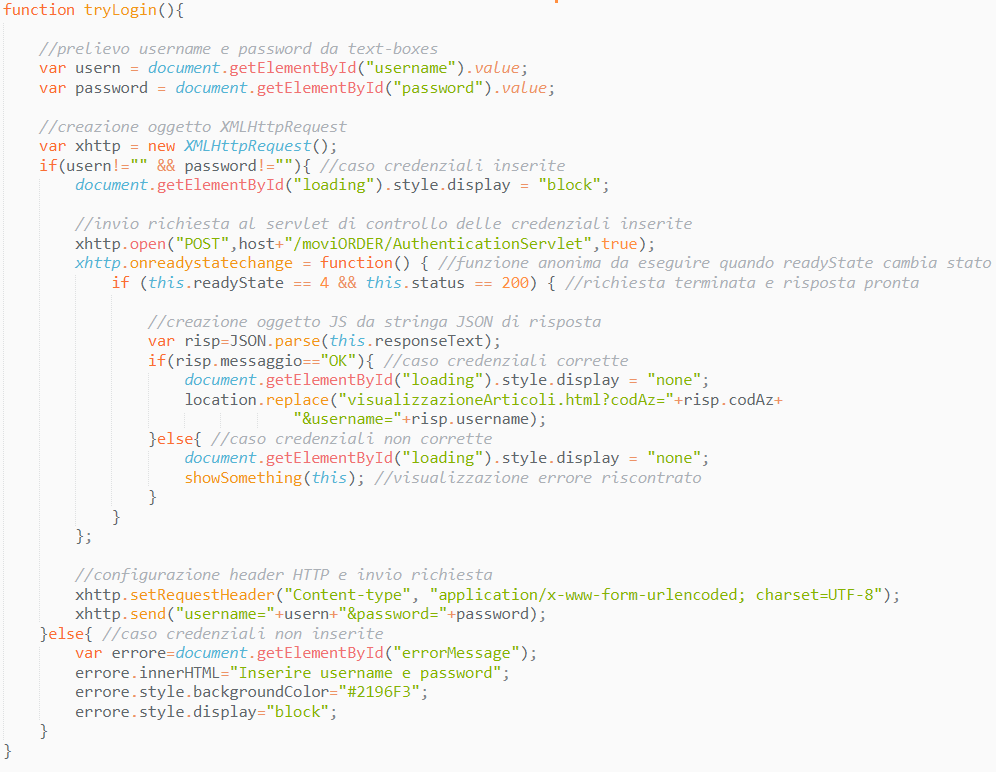
\includegraphics[width=\columnwidth]{codice/ajax} 
    \caption{Esempio di invio di una richiesta \textit{HTTP} tramite \textit{AJAX}}
\end{figure}

\subsubsection{API del servizio web} \label{api}

In questa sezione viene presentata la \textit{API} del servizio web di \textit{moviORDER}. In particolare, per ogni \textit{end-point} (\textit{servlet}) vengono specificati:
\begin{itemize}
	\item \textbf{indirizzo}: indirizzo tramite il quale è possibile raggiungere l'\textit{end-point};
	\item \textbf{input}: costituito dai parametri inviati al servizio web tramite una richiesta \textit{HTTP};
	\item \textbf{output}: costituito da una stringa in formato \textit{JSON} che presenta struttura diversa a seconda dell'\textit{end-point} che gestisce la richiesta;
	\item \textbf{descrizione}.
\end{itemize}

\myparagraph{Servizio di autenticazione}

\begin{itemize}
	\item \textbf{Indirizzo}: /AuthenticationServlet;
	\item \textbf{Input}: il \textit{servlet} richiede i seguenti parametri:
		\begin{itemize}
			\item \textit{username}: è la \textit{username} inserita dall'utente in fase di login;
			\item \textit{password}: è la password inserita dall'utente in fase di login.
		\end{itemize}
	\item \textbf{Output}: le possibili risposte del \textit{servlet} sono le seguenti:
		\begin{itemize}
			\item codice azienda e \textit{username} dell'utente nel caso in cui \textit{username} e password passati come parametro corrispondono ad un utente presente in \textit{database};
			\item un messaggio d'errore nel caso in cui le credenziali sono scorrette o l'utente è stato bloccato. 
		\end{itemize}
		\item \textbf{Descrizione}: questo \textit{servlet} rappresenta il servizio di autenticazione di \textit{moviORDER}. Ricevuti i parametri, il \textit{servlet} cerca la \textit{username} dell'utente nel \textit{database} e, nel caso in cui questa fosse presente, procede nel cercare la password corrispondente. Nel caso in cui \textit{username} e password passati siano quelli corretti, il \textit{servlet} restituisce una stringa \textit{JSON} contenente il codice azienda e la \textit{username} dell'utente che ha cercando di loggarsi. Nel caso in cui le credenziali non siano corrette, oppure l'utente è stato bloccato, viene restituito un messaggio d'errore.
\end{itemize}

\myparagraph{Servizio di verifica di connessione con il \textit{database}}

\begin{itemize}
	\item \textbf{Indirizzo}: /CheckConnectionURL;
	\item \textbf{Input}: il \textit{servlet} richiede i seguenti parametri:
		\begin{itemize}
			\item \textit{codice azienda}: è il codice azienda dell'azienda cliente di \visione{} della quale si vuole verificare la presenza del \textit{database}.
		\end{itemize}
	\item \textbf{Output}: le possibili risposte del \textit{servlet} sono le seguenti:
		\begin{itemize}
			\item un messaggio positivo nel caso in cui il \textit{database} dell'azienda corrispondente al codice inserito è raggiungibile;
			\item un messaggio negativo nel caso in cui il \textit{database} dell'azienda corrispondente al codice inserito non è raggiungibile.
		\end{itemize}
	\item \textbf{Descrizione}: questo \textit{servlet} si occupa di controllare se un \textit{database} aziendale è raggiungibile provando ad effettuare una \textit{query} su tale \textit{database}. Risponde positivamente nel caso in cui il \textit{database} dell'azienda corrispondente al codice inserito è raggiungibile (\textit{query} con un ritorno), mentre risponde negativamente nel caso in cui il \textit{database} non è raggiungibile (\textit{query} che ha sollevato un eccezione).
\end{itemize}

\myparagraph{Servizio di rimozione articoli dal carrello}

\begin{itemize}
	\item \textbf{Indirizzo}: /DeleteSelectedItems;
	\item \textbf{Input}: il \textit{servlet} richiede i seguenti parametri:
		\begin{itemize}
			\item \textit{lista di codici articolo}: è una lista dei codici articolo degli articoli che devono essere eliminati;
			\item \textit{username}: è la \textit{username} dell'utente che ha richiesto l'eliminazione degli articoli;
			\item \textit{path}: è la stringa di connessione al \textit{database} aziendale dell'utente autenticato.
		\end{itemize}
	\item \textbf{Output}: le possibili risposte del \textit{servlet} sono le seguenti:
		\begin{itemize}
			\item un messaggio positivo nel caso in cui la cancellazione è andata a buon fine;
			\item un messaggio negativo nel caso in cui la cancellazione non è andata a buon fine.
		\end{itemize}
	\item \textbf{Descrizione}: questo \textit{servlet} si occupa di eliminare dal \textit{database} aziendale dell'utente autenticato gli articoli che quest'ultimo ha richiesto di rimuovere dal carrello. Risponde positivamente nel caso in cui gli articoli sono stati rimossi correttamente dal \textit{database}, mentre risponde negativamente nel caso in cui gli articoli non sono stati rimossi dal \textit{database}.
\end{itemize}

\myparagraph{Servizio di ricerca di un codice a barre}

\begin{itemize}
	\item \textbf{Indirizzo}: /FindArticleBarCode;
	\item \textbf{Input}: il \textit{servlet} richiede i seguenti parametri:
		\begin{itemize}
			\item \textit{codice a barre}: è il codice a barre di un articolo del quale si vuole conoscere il codice articolo;
			\item \textit{path}: è la stringa di connessione al \textit{database} aziendale dell'utente autenticato.
		\end{itemize}
	\item \textbf{Output}: le possibili risposte del \textit{servlet} sono le seguenti:
		\begin{itemize}
			\item codice articolo corrispondente al \textit{barcode} passato come parametro nel caso in cui il \textit{barcode} corrisponde a quello di un articolo venduto dall'azienda;
			\item un messaggio negativo nel caso in cui il \textit{barcode} passato come parametro non corrisponde ad un articolo venduto dall'azienda.
		\end{itemize}
	\item \textbf{Descrizione}: questo \textit{servlet} si occupa di fornire il codice articolo dell'articolo corrispondente al codice a barre ricevuto come parametro, effettuando la ricerca del \textit{barcode} all'interno del \textit{database}. Nel caso in cui il codice a barre è presente all'interno del \textit{database} viene restituito il codice articolo corrispondente, mentre nel caso in cui non è presente viene restituito un messaggio negativo.
\end{itemize}

\myparagraph{Servizio di ricerca di un codice articolo}

\begin{itemize}
	\item \textbf{Indirizzo}: /FindArticleCode;
	\item \textbf{Input}: il \textit{servlet} richiede i seguenti parametri:
		\begin{itemize}
			\item \textit{codice articolo}: è il codice articolo o il \textit{barcode} di un articolo del quale si vuole verificare la presenza in \textit{database};
		\end{itemize}
	\item \textbf{Output}: le possibili risposte del \textit{servlet} sono le seguenti:
		\begin{itemize}
			\item codice articolo nel caso in cui l'articolo è presente in \textit{database};
			\item un messaggio negativo nel caso in cui l'articolo non è presente in \textit{database}.
		\end{itemize}
	\item \textbf{Descrizione}: questo \textit{servlet} si occupa di fornire il codice articolo dell'articolo corrispondente al codice articolo o al \textit{barcode} ricevuto come parametro, effettuando la ricerca del codice articolo o del \textit{barcode} all'interno del \textit{database}. Nel caso in cui il codice articolo o il \textit{barcode} passato come parametro corrisponde ad un articolo presente in \textit{database} viene restituito il codice articolo, mentre nel caso in cui non corrisponde ad un articolo presente in \textit{database} viene restituito un messaggio negativo.
\end{itemize}

\myparagraph{Servizio di prelievo informazioni di un articolo}

\begin{itemize}
	\item \textbf{Indirizzo}: /GetArticleDescNote;
	\item \textbf{Input}: il \textit{servlet} richiede i seguenti parametri:
		\begin{itemize}
			\item \textit{codice azienda}: è il codice azienda della quale l'utente autenticato è cliente;
			\item \textit{codice articolo}: è il codice articolo dell'articolo del quale si vogliono ottenere informazioni.
		\end{itemize}
	\item \textbf{Output}: questo \textit{servlet} può produrre un solo output poiché l'applicazione è stata implementata in modo che non ci siano casi negativi:
		\begin{itemize}
			\item descrizione, note, quantità minima ordinabile e step di incremento quantità per l'articolo corrispondente al codice articolo passato come parametro.
		\end{itemize}
	\item \textbf{Descrizione}: questo \textit{servlet} si occupa di fornire informazioni sull'articolo corrispondente al codice articolo passato come parametro. 
\end{itemize}

\myparagraph{Servizio di prelievo degli articoli in carrello}

\begin{itemize}
	\item \textbf{Indirizzo}: /GetArticlesByUsername;
	\item \textbf{Input}: il \textit{servlet} richiede i seguenti parametri:
		\begin{itemize}
			\item \textit{codice azienda}: è il codice azienda della quale l'utente autenticato è cliente;
			\item \textit{username}: è il nome utente dell'utente autenticato.
		\end{itemize}
	\item \textbf{Output}: le possibili risposte del \textit{servlet} sono le seguenti:
		\begin{itemize}
			\item array degli articoli nel carrello dell'utente autenticato, dove per ogni articolo vengono restituiti la quantità ordinata, il codice articolo e la descrizione dell'articolo;
			\item array vuoto nel caso in cui l'utente autenticato non presenta articoli in carrello.
		\end{itemize}
	\item \textbf{Descrizione}: questo \textit{servlet} si occupa di fornire la lista degli articoli in carrello per l'utente la quale \textit{username} è stata passata come parametro. Nel caso in cui l'utente presenta articoli in carrello viene restituita la lista degli articoli in carrello, mentre nel caso in cui non presenta articoli in carrello viene restituita una lista vuota.
\end{itemize}

\myparagraph{Servizio di prelievo di informazioni di un utente}

\begin{itemize}
	\item \textbf{Indirizzo}: /GetNameByUsername;
	\item \textbf{Input}: il \textit{servlet} richiede i seguenti parametri:
		\begin{itemize}
			\item \textit{path}: è la stringa di connessione al \textit{database} aziendale dell'utente autenticato;
			\item \textit{username}: è il nome utente dell'utente autenticato.
		\end{itemize}
	\item \textbf{Output}: questo \textit{servlet} può produrre un solo output poiché l'applicazione è stata implementata in modo che non ci siano casi negativi:
		\begin{itemize}
			\item nome e ragione sociale dell'utente autenticato e codice documento e descrizione del documento da generare nel caso in cui l'utente invii un ordine.
		\end{itemize}
	\item \textbf{Descrizione}: questo \textit{servlet} si occupa di fornire informazioni sull'utente la cui \textit{username} è stata passata come parametro.
\end{itemize}

\myparagraph{Servizio di prelievo informazioni di un articolo in carrello}

\begin{itemize}
	\item \textbf{Indirizzo}: /GetTmpArticleData;
	\item \textbf{Input}: il \textit{servlet} richiede i seguenti parametri:
		\begin{itemize}
			\item \textit{path}: è la stringa di connessione al \textit{database} aziendale dell'utente autenticato;
			\item \textit{codice articolo}: è il codice articolo dell'articolo del quale si vogliono ottenere informazioni;
			\item \textit{username}: è il nome utente dell'utente autenticato.
		\end{itemize}
	\item \textbf{Output}: questo \textit{servlet} può produrre un solo output poiché l'applicazione è stata implementata in modo che non ci siano casi negativi:
		\begin{itemize}
			\item quantità e note dell'articolo nel carrello dell'utente autenticato corrispondente al codice articolo passato come parametro.
		\end{itemize}
	\item \textbf{Descrizione}: questo \textit{servlet} si occupa di fornire informazioni riguardati uno specifico articolo nel carrello dell'utente la quale \textit{username} è stata passata come parametro.
\end{itemize}

\myparagraph{Servizio di inserimento/modifica articolo}

\begin{itemize}
	\item \textbf{Indirizzo}: /InsertUpdateArticle;
	\item \textbf{Input}: il \textit{servlet} richiede i seguenti parametri:
		\begin{itemize}
			\item \textit{path}: è la stringa di connessione al \textit{database} aziendale dell'utente autenticato;
			\item \textit{query}: è una stringa contenente la \textit{query} di inserimento/modifica di un articolo.
		\end{itemize}
	\item \textbf{Output}: le possibili risposte del \textit{servlet} sono le seguenti:
		\begin{itemize}
			\item un messaggio positivo nel caso in cui la \textit{query} di inserimento/modifica articolo è andata a buon fine;
			\item un messaggio negativo nel caso in cui la \textit{query} di inserimento/modifica articolo non è andata a buon fine.
		\end{itemize}
	\item \textbf{Descrizione}: questo \textit{servlet} si occupa di inserire o modificare un articolo nel carrello dell'utente autenticato. L'inserimento e la modifica avvengono mediante l'utilizzo dello stesso \textit{servlet} poiché la \textit{query} da eseguire sul \textit{database}, che può essere di tipo \textit{INSERT} o \textit{UPDATE}, viene passata come parametro. Nel caso in cui la \textit{query} viene eseguita in modo corretto sul \textit{database} viene restituito un messaggio positivo, mentre nel caso in cui non viene eseguita viene restituito un messaggio negativo.
\end{itemize}

\myparagraph{Servizio di invio di un ordine}

\begin{itemize}
	\item \textbf{Indirizzo}: /SendOrder;
	\item \textbf{Input}: il \textit{servlet} richiede i seguenti parametri:
		\begin{itemize}
			\item path: è la stringa di connessione al \textit{database} aziendale dell'utente autenticato;
			\item codici articolo: è la lista dei codici degli articoli che l'utente autenticato ha ordinato;
			\item \textit{username}: è il nome utente dell'utente autenticato;
			\item ragione sociale: è la ragione sociale dell'utente autenticato;
			\item nome: è il nome dell'utente autenticato;
			\item codice documento: è il codice del documento che deve essere generato con l'ordine;
			\item data: è la data d'invio dell'ordine;
			\item note: sono le note inserite dall'utente in fase di invio dell'ordine;
			\item codice azienda: è il codice azienda della quale l'utente autenticato è cliente.
		\end{itemize}
	\item \textbf{Output}: le possibili risposte del \textit{servlet} sono le seguenti:
		\begin{itemize}
			\item un messaggio positivo nel caso in cui l'ordine è stato inviato con successo;
			\item un messaggio negativo nel caso in cui l'ordine non è stato inviato con successo.
		\end{itemize}
	\item \textbf{Descrizione}: questo \textit{servlet} si occupa di registrare sul \textit{database} un ordine contenente gli articoli passati come parametro. Il resto dei parametri passati viene utilizzato per inviare una mail di conferma all'utente autenticato e all'azienda presso cui l'utente è cliente. Nel caso in cui la registrazione dell'ordine sul \textit{database} avvenga correttamente viene restituito un messaggio positivo, mentre nel caso in cui non avvenga correttamente viene restituito un messaggio negativo.
\end{itemize}

\subsection{JDBC}

In questa sezione viene presentato l'utilizzo della \textit{Java Database Connectivity API} nella realizzazione del servizio web.

\subsubsection{Driver JDBC}

Un driver \textit{JDBC} è una componente software che permette ad un'applicazione \textit{Java} di interagire con un \textit{database}. Per supportare la connessione a singoli \textit{database}, \textit{JDBC} (\textit{Java Database Connectivity API}) richiede i driver per ogni \textit{database}. Il driver permette la connessione con il \textit{database} e implementa il protocollo di trasferimento di \textit{query} e risultati tra il \textit{client} e il \textit{database}. Poiché per l'implementazione del \textit{database} è stato utilizzato \textit{SQL Server} si sono dovuti utilizzare i driver \textit{JDBC} per tale \textit{database}.

\subsubsection{Classe DatabaseConnection} \label{dbconnect}

Per lo sviluppo del servizio web è stata realizzata la classe \textit{DatabaseConnection} appartenente al \textit{package} \textit{dbConnection}. Tale classe fornisce un'interfaccia utilizzabile per la gestione dell'interazione con un \textit{database} di tipo \textit{SQL Server}. In questa sezione vengono presentati i metodi che costituiscono tale interfaccia.

\myparagraph{Costruttori}

La classe presenta due metodi costruttori:
\begin{itemize}
	\item \textit{public DatabaseConnection(String u, String user, String psw, String db)}: costruisce un oggetto \textit{DatabaseConnection} a partire dall'\textit{URL} del \textit{server} in cui è presente il \textit{database}, la \textit{username} e la password di accesso al \textit{database}, e il nome del \textit{database} al quale si desidera connettesi;
	\item \textit{public DatabaseConnection(String dbConnectionString)}: costruisce un oggetto \textit{DatabaseConnection} a partire dalla stringa di connessione ad uno specifico \textit{database}.
\end{itemize}
Il formato della stringa di connessione ad un \textit{database} è il seguente: \textit{indirizzoServer;databaseName=nomeDb;user=u;password=psw}, dove:
\begin{itemize}
	\item \textit{indirizzoServer}: è l'indirizzo IP pubblico del \textit{server} contenente il \textit{database} al quale si desidera connettersi. Nel caso del progetto potrebbe essere l'indirizzo del \textit{server} di un'azienda esterna che desidera utilizzare il proprio \textit{database} per l'interazione;
	\item \textit{nomeDb}: è il nome del \textit{database} al quale si desidera connettersi;
	\item \textit{u}: è il nome utente per l'accesso al \textit{database};
	\item \textit{psw}: è la password per l'accesso al \textit{database}.
\end{itemize}
Viene di seguito presentato, a titolo d'esempio, il codice \textit{Java} che implementa il metodo \textit{public DatabaseConnection(String dbConnectionString)}. Il metodo si occupa di splittare la stringa di connessione passata come parametro per ottenere i dati utili alla costruzione dell'oggetto \textit{DatabaseConnection}.

\begin{figure}[!h] 
    \centering 
    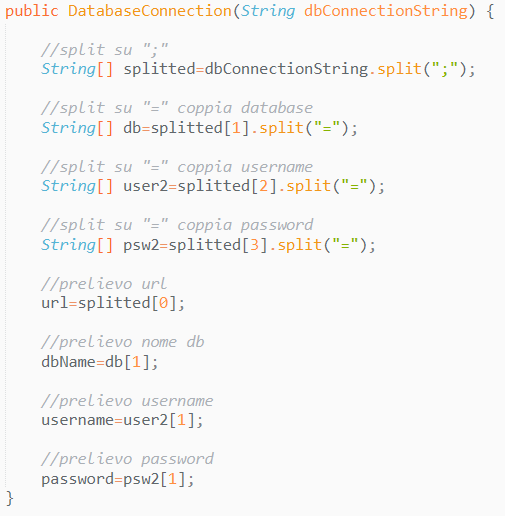
\includegraphics[height=8cm,width=0.8\columnwidth]{codice/databaseCostruttore} 
    \caption{Metodo costruttore della classe \textit{DatabaseConnection}}
\end{figure}

\myparagraph{Metodo \textit{connectToDb()}}

Tale metodo si occupa di instaurare la connessione con il \textit{database} desiderato. Per far questo, configura i driver \textit{JDBC} e costruisce l'\textit{URL} di connessione al \textit{database} tramite i dati contenuti nell'oggetto d'invocazione. Il metodo potrebbe sollevare un'eccezione di tipo \textit{ClassNotFoundException} nel caso in cui la classe utilizzata per i driver \textit{JDBC} sia inesistente o non sia stata importata all'interno del progetto. Viene di seguito fornito, a titolo d'esempio, il codice del metodo \textit{connectToDb()}.

\begin{figure}[!h] 
    \centering 
    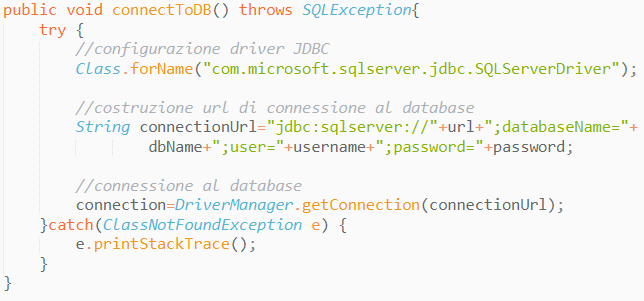
\includegraphics[width=\columnwidth]{codice/connessionedb} 
    \caption{Metodo \textit{connectToDb()} della classe \textit{DatabaseConnection}}
\end{figure}

\myparagraph{Altri metodi}

Sono stati implementati altri metodi di complessità inferiore. Per questo motivo ne viene presentata solamente una breve descrizione:
\begin{itemize}
	\item \textit{doQuery(query)}: questo metodo permette di eseguire una \textit{query} di tipo \textit{SELECT} sul \textit{database}. Restituisce il \textit{ResultSet} contenente il risultato della \textit{query};
	\item \textit{doUpdateQuery(query)}: questo metodo permette di eseguire una \textit{query} di tipo \textit{INSERT}, \textit{UPDATE} o \textit{DELETE} sul \textit{database}. Restituisce il numero di righe inserite, modificate o cancellate;
	\item \textit{closeConnection()}: questo metodo permette di eseguire il processo di disconnessione dal \textit{database}.
\end{itemize}

\subsection{Classi utilità}

Per lo sviluppo del servizio web è stato necessario implementare due classi utilità. In questa sezione ne viene presentata brevemente l'implementazione. Tali classi appartengono al \textit{package} \textit{utility}.

\subsubsection{Classe GetParam}

La classe \textit{GetParam} si occupa di restituisce un campo statico contenente la stringa di connessione al \textit{database} \textit{CommonDb} dell'applicazione \textit{moviORDER}. Come detto precedentemente, questo \textit{database} contiene tutti i dati di autenticazione degli utenti di \textit{moviORDER}. Poiché tale stringa di connessione viene utilizzata frequentemente all'interno del servizio web, si è deciso di inserirla in un unico punto del servizio, in modo da evitare la modifica di più file nel caso in cui essa cambi.

\subsubsection{Classe MailUtility}

La classe \textit{MailUtility} fornisce un'interfaccia per l'invio di e-mail. È stato necessario implementare tale classe poiché è stato richiesto di inviare una mail di conferma all'utente autenticato e all'azienda presso cui l'utente è cliente nel momento in cui un ordine viene registrato. La classe presenta un costruttore che richiede i parametri per la configurazione di un \textit{server SMTP}:
\begin{itemize}
	\item \textbf{host}: è l'indirizzo IP dell'\textit{host} su cui è installato il \textit{server SMTP};
	\item \textbf{post}: è il numero di porta dell'\textit{host} su cui è installato il \textit{server SMTP};
	\item \textbf{username}: è il nome utente di accesso al \textit{server SMTP};
	\item \textbf{password}: è la password di accesso al \textit{server SMTP}.
\end{itemize}
Il metodo \textit{sendMail()} si occupa di configurare e inviare una mail all'utente che ha effettuato l'ordine e all'azienda presso cui l'utente è cliente. Per far questo, il metodo richiede:
\begin{itemize}
	\item indirizzo e-mail dell'utente;
	\item indirizzo e-mail dell'azienda;
	\item indirizzo e-mail del mittente;
	\item oggetto della e-mail;
	\item testo della e-mail: è una tabella scritta in codice \textit{HTML} contenente i dati degli articoli ordinati.
\end{itemize}
Viene di seguito fornito, a titolo d'esempio, il codice \textit{Java} che implementa il metodo \textit{sendMail()}.

\newpage

\begin{figure}[!h] 
    \centering 
    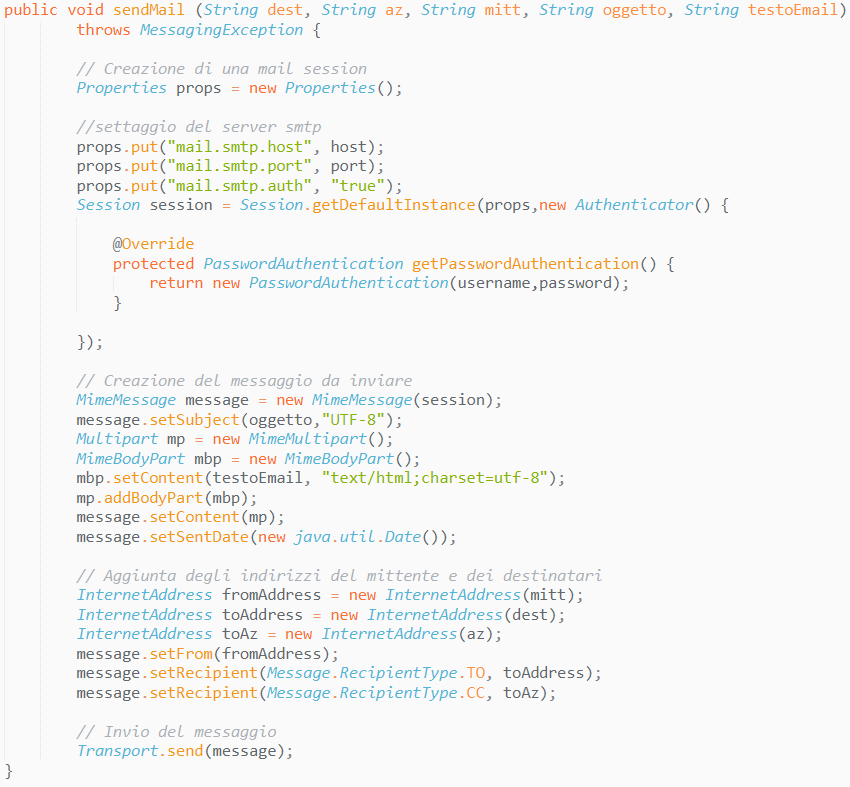
\includegraphics[width=\columnwidth]{codice/mail} 
    \caption{Metodo \textit{sendMail()} della classe \textit{MailUtility}}
\end{figure}

\section{Logica applicativa}

In questa sezione vengono presentati gli aspetti più interessanti riguardanti la codifica della logica applicativa di \textit{moviORDER}. La sezione si incentra sui meccanismi di integrazione dei \textit{plugin} \textit{PhoneGap} con il codice \textit{Javascript} della logica applicativa.

\subsection{Plugin di PhoneGap}

Un \textit{plugin} è un pacchetto di codice che permette al visualizzatore web di \textit{Cordova}, il quale renderizza l'applicazione, di comunicare con la piattaforma nativa sulla quale viene eseguito. I \textit{plugin} forniscono accesso alle funzionalità del dispositivo che normalmente non sono disponibili per le applicazioni \textit{web-based}. Tutte le \textit{API} di \textit{Cordova} sono implementate tramite \textit{plugin}. Essi sono composti da un'unica interfaccia \textit{JavaScript} che astrae le differenti implementazioni in codice nativo delle funzionalità fornite dal \textit{plugin}. In fase di \textit{build} dell'applicazione il codice \textit{JavaScript} dei \textit{plugin} viene quindi convertito nel codice nativo della piattaforma sulla quale si sta distribuendo l'applicazione.

\subsection{Installazione dei plugin}

Tramite \textit{PhoneGap CLI}, interfaccia a linea di comando precedentemente descritta, è possibile aggiungere \textit{plugin} alla configurazione del progetto \textit{PhoneGap}. È sufficiente lanciare la CLI dalla cartella principale del progetto ed eseguire il comando \textit{phonegap plugin add nomePlugin}, dove \textit{nomePlugin} è il nome del \textit{plugin} che si desidera scaricare ed installare (es. \textit{cordova-plugin-whitelist}).

\subsection{Premesse all'utilizzo dei plugin}

Per poter utilizzare efficacemente i \textit{plugin} è necessario predisporre il codice \textit{JavaScript} al loro utilizzo. In particolare sono necessari due accorgimenti che vengono di seguito presentati.

\subsubsection{Inclusione di cordova.js}

Ogni file della logica applicativa di \textit{moviORDER} che utilizza dei \textit{plugin} deve includere il file \textit{cordova.js}. Questo file \textit{JavaScript} permette il funzionamento dei \textit{plugin} utilizzati all'interno della logica. Se si utilizzasse un \textit{plugin} senza aver importato tale file, la console darebbe il seguente errore: ``\textit{Cordova} in not available, Make sure to include cordova.js''.

\subsubsection{Evento deviceready}

L'evento \textit{deviceready} è essenziale in ogni applicazione \textit{PhoneGap} poiché segnala il corretto caricamento delle \textit{API} di \textit{Cordova} sul dispositivo. Se l'evento non venisse atteso prima di utilizzare un \textit{plugin}, si rischierebbe che l'applicazione effettui una chiamata ad una funzione \textit{JavaScript} di \textit{Cordova} prima che il corrispondente codice nativo per il dispositivo diventi disponibile. L'evento \textit{deviceready} viene lanciato nel momento in cui \textit{Cordova} è stato completamente caricato. Quindi dopo aver atteso l'evento, è possibile effettuare chiamate alle \textit{API} di \textit{Cordova} in completa sicurezza. Per attendere l'evento è sufficiente inserire un listener nel codice \textit{JavaScript}. Viene di seguito fornito, a scopo illustrativo, un esempio di codice \textit{JavaScript} che implementa l'attesa di tale evento.

\begin{figure}[!h] 
    \centering 
    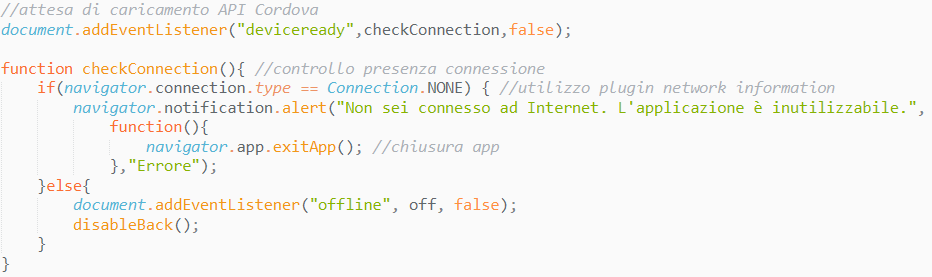
\includegraphics[width=\columnwidth]{codice/deviceready} 
    \caption{Esempio di codice \textit{JavaScript} che attende l'evento \textit{deviceready}}
\end{figure}

\subsection{Plugin utilizzati}

In questa sezione vengono presentati i \textit{plugin} \textit{PhoneGap} utilizzati nella realizzazione della logica applicativa di \textit{moviORDER}. Per ogni \textit{plugin} vengono messi in evidenzia vantaggi e svantaggi (se presenti) nell'utilizzo e un esempio di utilizzo.

\subsubsection{Dialogs plugin}

Il \textit{plugin} \textit{dialogs} fornisce accesso all'interfaccia grafica nativa degli elementi \textit{dialog} tramite l'utilizzo dell'oggetto \textit{navigator.notification}. Questo \textit{plugin} è stato utilizzato per convertire gli \textit{alert box} delle usuali pagine web in \textit{dialog} nativi per l'ambiente mobile. Sono stati utilizzati i seguenti metodi:
\begin{itemize}
	\item \textit{alert()}: visualizza un \textit{dialog} con un messaggio di allerta preimpostato. Il metodo richiede i seguenti parametri:
	\begin{itemize}
		\item \textit{message}: è il messaggio visualizzato nel \textit{dialog};
		\item \textit{callback}: è una funzione anonima di \textit{callback} da eseguire quando viene premuto il pulsante nel \textit{dialog};
		\item \textit{title}: è il titolo del \textit{dialog};
		\item \textit{buttonName}: è l'etichetta del pulsante nel \textit{dialog}.
	\end{itemize}
	\item \textit{confirm()}: visualizza un \textit{dialog} per chiedere conferma di un'azione. Il metodo richiede i seguenti parametri:
	\begin{itemize}
		\item \textit{message}: è il messaggio visualizzato nel \textit{dialog} di conferma;
		\item \textit{callback}: è una funzione anonima di \textit{callback} da eseguire nel caso in cui il bottone di conferma viene premuto;
		\item \textit{title}: è il titolo del \textit{dialog} di conferma;
		\item \textit{buttonLabels}: sono le etichette dei vari bottoni presenti nel \textit{dialog} di conferma. Solitamente sono ``OK'' e ``Annulla''.
	\end{itemize}
\end{itemize}

Senza l'utilizzo di questo \textit{plugin} non sarebbe stato possibile modificare il titolo e i bottoni del \textit{dialog} poiché per motivi di sicurezza \textit{JavaScript} non permette tale modifica. Inoltre la visualizzazione del \textit{dialog} non sarebbe stata quella desiderata, ovvero la visualizzazione nativa. 

Vengono di seguito forniti, a scopo illustrativo, un esempio di codice \textit{JavaScript} che non utilizza il \textit{plugin} e un esempio che lo utilizza. Per ognuno degli esempi viene mostrato uno \textit{screenshot} dell'output risultante che, nel primo caso sarà un comune \textit{alert} e nel secondo un \textit{dialog} nativo.

\begin{figure}[!h] 
    \centering 
    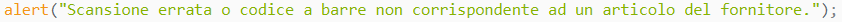
\includegraphics[width=\columnwidth]{codice/alert} 
    \caption{Esempio di codice \textit{JavaScript} che non utilizza il \textit{plugin} \textit{dialogs}}
\end{figure}

\newpage

\begin{figure}[!h] 
    \centering 
    \includegraphics[width=0.4\columnwidth]{codice/imgalert} 
    \caption{Esempio di visualizzazione scorretta - \textit{alert}}
\end{figure}

\begin{figure}[!h] 
    \centering 
    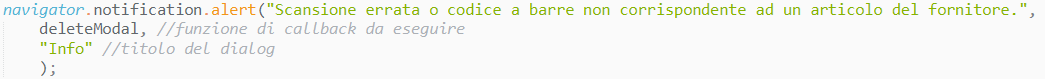
\includegraphics[width=\columnwidth]{codice/dialog} 
    \caption{Esempio di codice \textit{JavaScript} che utilizza il \textit{plugin} \textit{dialogs}}
\end{figure}

\begin{figure}[!h] 
    \centering 
    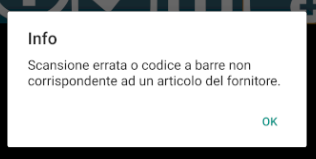
\includegraphics[width=0.4\columnwidth]{codice/imgDialog} 
    \caption{Esempio di visualizzazione corretta - \textit{dialog}}
\end{figure}

\subsubsection{Network information plugin}

Il \textit{plugin} \textit{network information} fornisce una moderna implementazione della \textit{Network Information API}. Essa fornisce informazioni riguardanti la rete cellulare e Wi-Fi del dispositivo e permette di capire se il dispositivo presenta una connessione ad Internet. Più precisamente, il \textit{plugin} fornisce un'interfaccia \textit{JavaScript} che astrae il codice nativo utilizzato per monitorare la rete del dispositivo. \textit{Navigator.connection} è l'oggetto che permette di acquisire le informazioni appena descritte. La proprietà \textit{type} è stata utilizzata per comprendere in modo veloce lo stato della connessione del dispositivo e la tipologia di connessione attiva. Essa può assumere i seguenti valori:
\begin{itemize}
	\item \textit{Connection.UNKNOWN}: tipologia di rete sconosciuta;
	\item \textit{Connection.ETHERNET}: dispositivo connesso alla rete via cavo \textit{ethernet};
	\item \textit{Connection.WIFI}: dispositivo connesso ad una rete \textit{Wi-Fi};
	\item \textit{Connection.CELL\_2G}: dispositivo connesso ad una rete cellulare di tipo \textit{2G};
	\item \textit{Connection.CELL\_3G}: dispositivo connesso ad una rete cellulare di tipo \textit{3G};
	\item \textit{Connection.CELL\_4G}: dispositivo connesso ad una rete cellulare di tipo \textit{4G};
	\item \textit{Connection.CELL}: dispositivo connesso ad una rete cellulare la cui tipologia non è identificabile;
	\item \textit{Connection.NONE}: dispositivo non connesso alla rete.
\end{itemize}
Un limite di questa proprietà è presente in ambiente \textit{iOS}, infatti non è possibile identificare nessun tipo di rete cellulare alla quale il dispositivo è connesso. Per questo, in ambiente \textit{iOS}, si è dovuta utilizzare la proprietà \textit{onLine} dell'oggetto \textit{navigator}.

All'oggetto \textit{navigator.connection} sono associate due tipologie di evento:
\begin{itemize}
	\item \textit{offline}: evento lanciato quando un dispositivo precedentemente collegato ad Internet perde la connessione e l'applicazione non è più in grado di accedere alla rete. In particolare, viene lanciato esattamente quando il valore della proprietà \textit{type} diventa \textit{Connection.NONE};
	\item \textit{online}: evento lanciato quando un dispositivo precedentemente scollegato dalla rete riceve la connessione permettendo all'applicazione di accedere ad Internet. In particolare, viene lanciato esattamente quando il valore della proprietà \textit{type} cambia da \textit{NONE} ad un altro valore.
\end{itemize}
Il \textit{plugin} \textit{network information} è stato utilizzato per chiudere \textit{moviORDER} nel caso in cui venisse aperta mentre il dispositivo è offline. L'evento \textit{offline} ha permesso di visualizzare messaggi relativi allo stato della connessione. Più precisamente, nel caso in cui il dispositivo perdesse la connessione durante l'utilizzo dell'applicazione viene visualizzato un messaggio che notifica all'utente che l'applicazione è inutilizzabile.

Vengono di seguito forniti, a scopo illustrativo, degli esempi di codice \textit{JavaScript} che utilizzano l'oggetto \textit{network.connection} ed in particolare la proprietà \textit{type} e l'evento \textit{offline}.

\begin{figure}[!h] 
    \centering 
    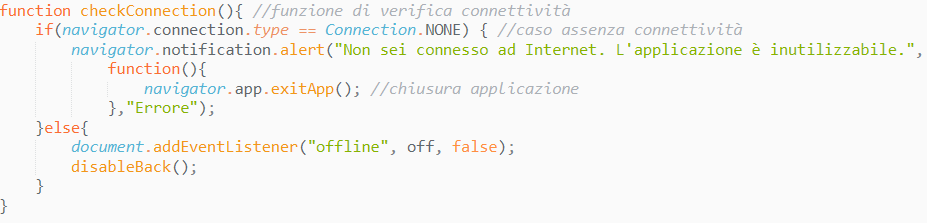
\includegraphics[width=\columnwidth]{codice/type} 
    \caption{Esempio di utilizzo della proprietà \textit{type}}
\end{figure}

\begin{figure}[!h] 
    \centering 
    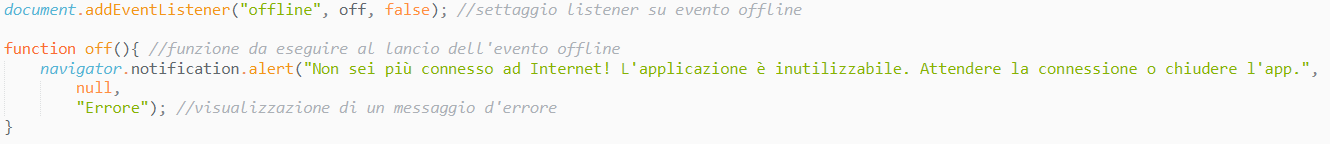
\includegraphics[width=\columnwidth]{codice/offline} 
    \caption{Esempio di utilizzo dell'evento \textit{offline}}
\end{figure}

\subsubsection{Barcode scanner plugin}

Il \textit{plugin} \textit{barcode scanner} fornisce un'interfaccia \textit{JavaScript} che astrae il codice nativo che permette di effettuare la scansione di un codice a barre da un qualsiasi dispositivo dotato di fotocamera. Il \textit{plugin} crea l'oggetto \textit{cordova.plugin.barcodeScanner} che presenta il metodo \textit{scan(success, fail, settings)}. \textit{Success} è una funzione di \textit{callback} che viene eseguita quando la scansione del codice a barre va a buon fine. \textit{Fail} è una funzione di \textit{callback} che viene eseguita quando la scansione del codice a barre non va a buon fine. \textit{Settings} è una variabile contenente un insieme di impostazioni per l'utilizzo del \textit{plugin}, quali:
\begin{itemize}
	\item \textit{preferFrontCamera}: permette di preferire la fotocamera frontale a quella posteriore per la scansione del codice a barre;
	\item \textit{showFlipCameraButton}: permette di visualizzare il bottone per il cambio della fotocamera;
	\item \textit{showTorchButton}: permette di visualizzare il bottone per l'attivazione del flash;
	\item \textit{torchOn}: permette di attivare il flash di default;
	\item \textit{saveHistory}: permette il salvataggio della cronologia dei codici scansionati;
	\item \textit{prompt}: permette la visualizzazione di un messaggio per aiutare l'utente nell'esecuzione della scansione;
	\item \textit{resultDisplayDuration}: permette la visualizzare di un testo per un determinato numero di secondi nel caso in cui un codice a barre viene captato;
	\item \textit{formats}: permette di impostare la tipologia di codici a barre che devono essere captati;
	\item \textit{orientation}: permette di impostare l'orientamento del dispositivo durante la scansione del codice a barre;
	\item \textit{disableAnimations}: permette la disattivazione di ogni tipo di animazione durante la scansione del codice a barre;
	\item \textit{disableSuccessBeep}: permette di disabilitare l'emissione del suono acustico nel caso in cui un codice a barre viene captato.
\end{itemize}
In ambiente iOS, per poter utilizzare il \textit{plugin}, è necessario aggiungere una \textit{NSCameraUsageDescription} al file \textit{Info.plist}. \textit{NSCameraUsageDescription} descrive la ragione per la quale l'applicazione accede alla fotocamera dell'utente. Quando il sistema operativo richiede all'utente di permettere l'accesso, la stringa inserita nella \textit{NSCameraUsageDescription} viene visualizzata sul \textit{dialog}. Se non viene fornita la descrizione di utilizzo, l'applicazione crescerà prima della visualizzazione del \textit{dialog}. Inoltre, Apple rifiuta le applicazioni che accedono a dati privati senza fornire una descrizione di utilizzo. 

Il \textit{plugin} ha funzionato perfettamente in ambiente \textit{Android} ma ha presentato alcuni problemi in ambiente \textit{iOS}. Nei dispositivi con una fotocamera mediocre le scansioni richiedevano più tempo del previsto, alcune volte anche minuti. Per risolvere il problema si è dovuto modificare il codice nativo della versione \textit{iOS} dell'applicazione. Il problema veniva riscontrato perché il codice differenziava il processo di scansione a seconda della qualità rilevata della fotocamera del dispositivo. Per cellulari con fotocamera mediocre veniva fatta una valutazione troppo ottimistica e per questo si è dovuto modificare il codice in modo da rendere il processo di scansione uguale per tutte le fotocamere. Dopo vari test si è potuto osservare che la soluzione migliore era l'utilizzo del processo di scansione per fotocamere di qualità media. Viene di seguito fornito, a scopo illustrativo, il codice \textit{Objective-C++} che si occupa di settare il processo di scansione.

\begin{figure}[!h] 
    \centering 
    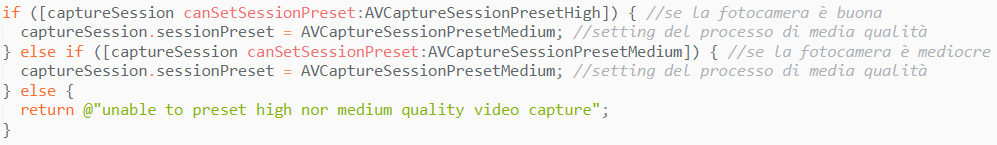
\includegraphics[width=\columnwidth]{codice/scan} 
    \caption{Codice \textit{Objective-C++} per il settaggio del processo di scansione}
\end{figure}

\newpage

Viene di seguito fornito, a scopo illustrativo, il codice \textit{JavaScript} della logica di \textit{moviORDER} che utilizza il \textit{plugin} \textit{barcode scanner}.

\begin{figure}[!h] 
    \centering 
    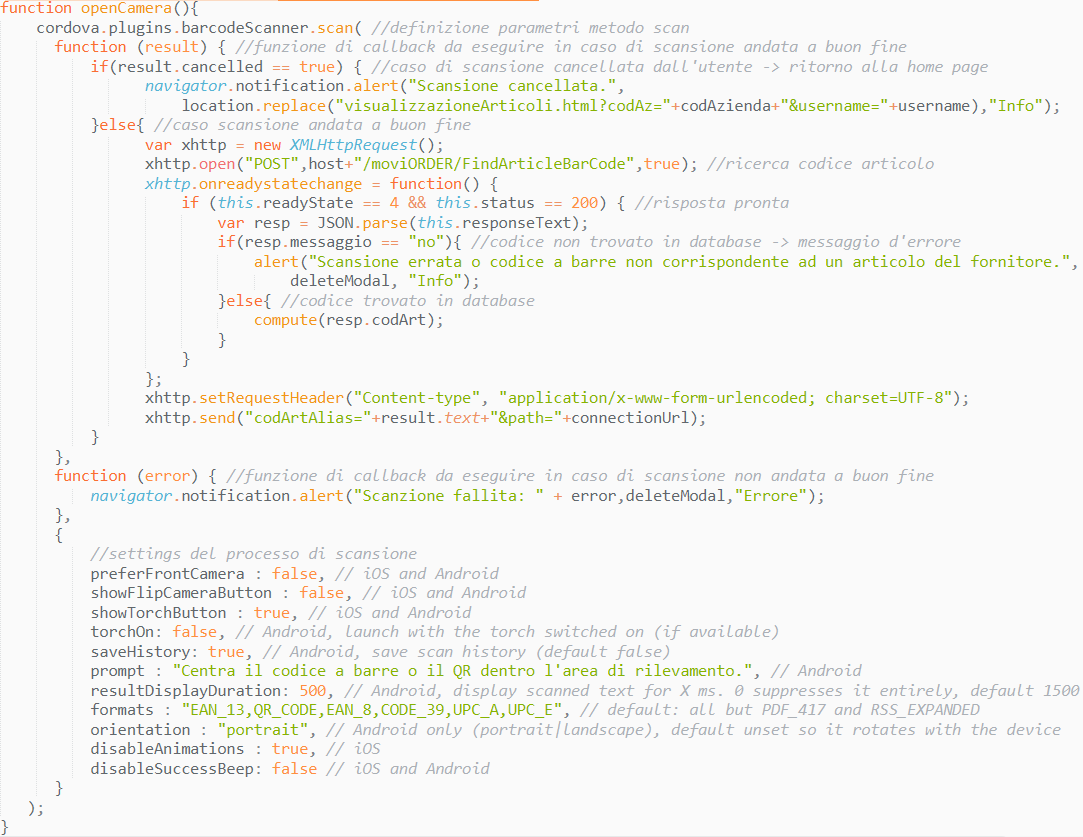
\includegraphics[width=\columnwidth]{codice/scan2} 
    \caption{Codice \textit{JavaScript} che utilizza il \textit{plugin} \textit{barcode scanner}}
\end{figure}

\newpage

\section{Interfaccia grafica}

In questa sezione vengono presentati gli aspetti più interessanti riguardanti la codifica dell'interfaccia grafica di \textit{moviORDER}. In particolare, vengono presentate le possibili interazioni dell'utente con le interfacce. Nell'ultima sezione vengono fatte delle considerazioni sullo sviluppo dell'interfaccia.

\subsection{Schermata di login}

\begin{figure}[!h] 
    \centering 
    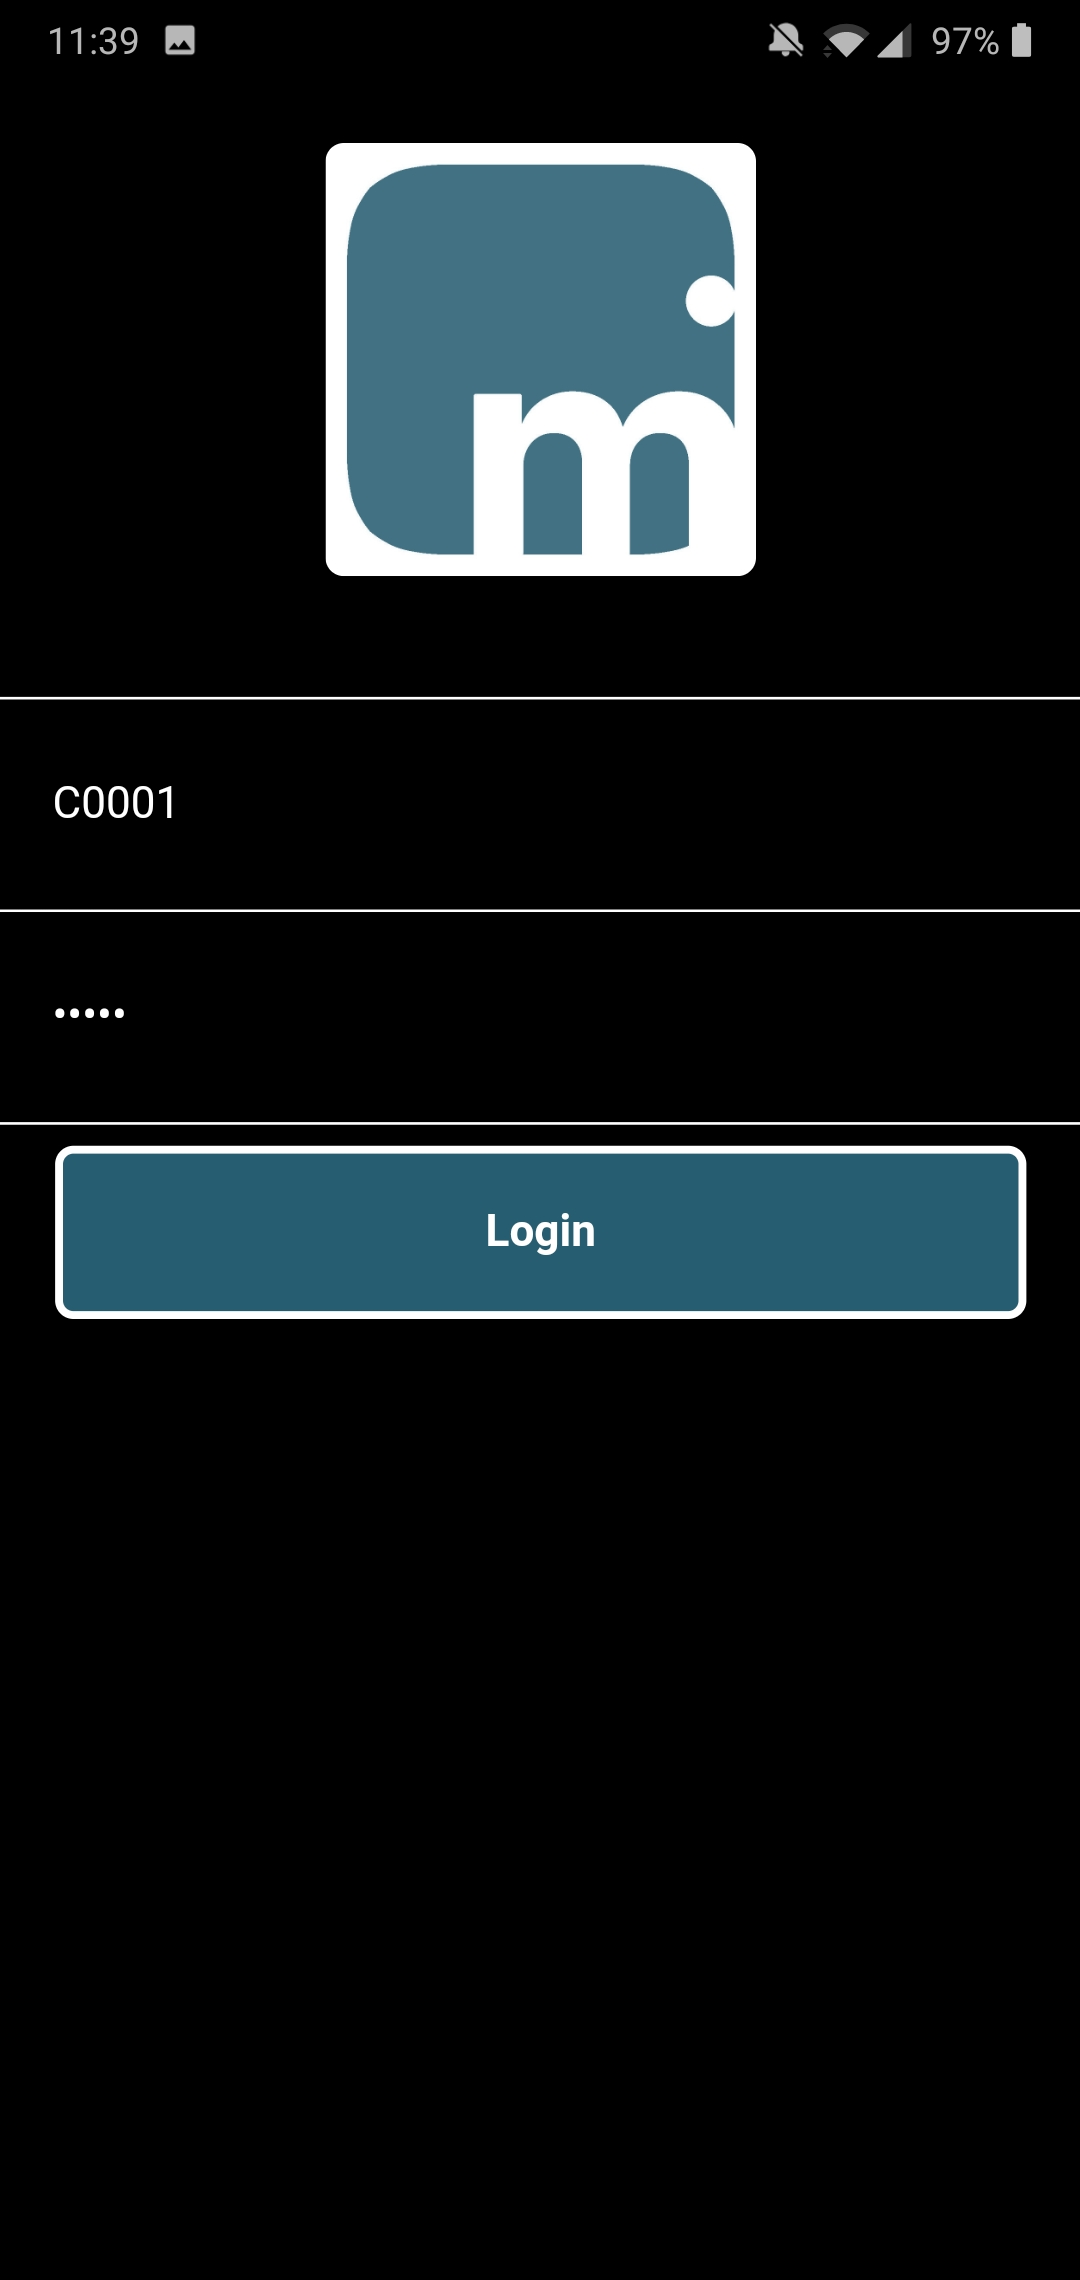
\includegraphics[width=0.4\columnwidth]{interfaccia/login} 
    \caption{Schermata di login}
\end{figure}

Tramite la schermata di login, un qualsiasi utente in possesso di credenziali di accesso può accedere a \textit{moviORDER}. Per tentare l'accesso, è necessario inserire \textit{username} e password e premere sul pulsante di login. Se l'utente ha inserito credenziali corrette viene aperta la \textit{home page} dell'applicazione, mentre se le credenziali non dovessero essere corrette viene visualizzato un messaggio d'errore. Il messaggio d'errore è esplicativo dell'errore riscontrato e i possibili errori sono:
\begin{itemize}
	\item le credenziali non sono state inserite;
	\item la \textit{username} inserita è inesistente;
	\item la password inserita non è corretta;
	\item le credenziali inserite sono corrette ma l'utente è stato bloccato dall'azienda.
\end{itemize}

\subsection{Home page}

\begin{figure}[!h] 
    \centering 
    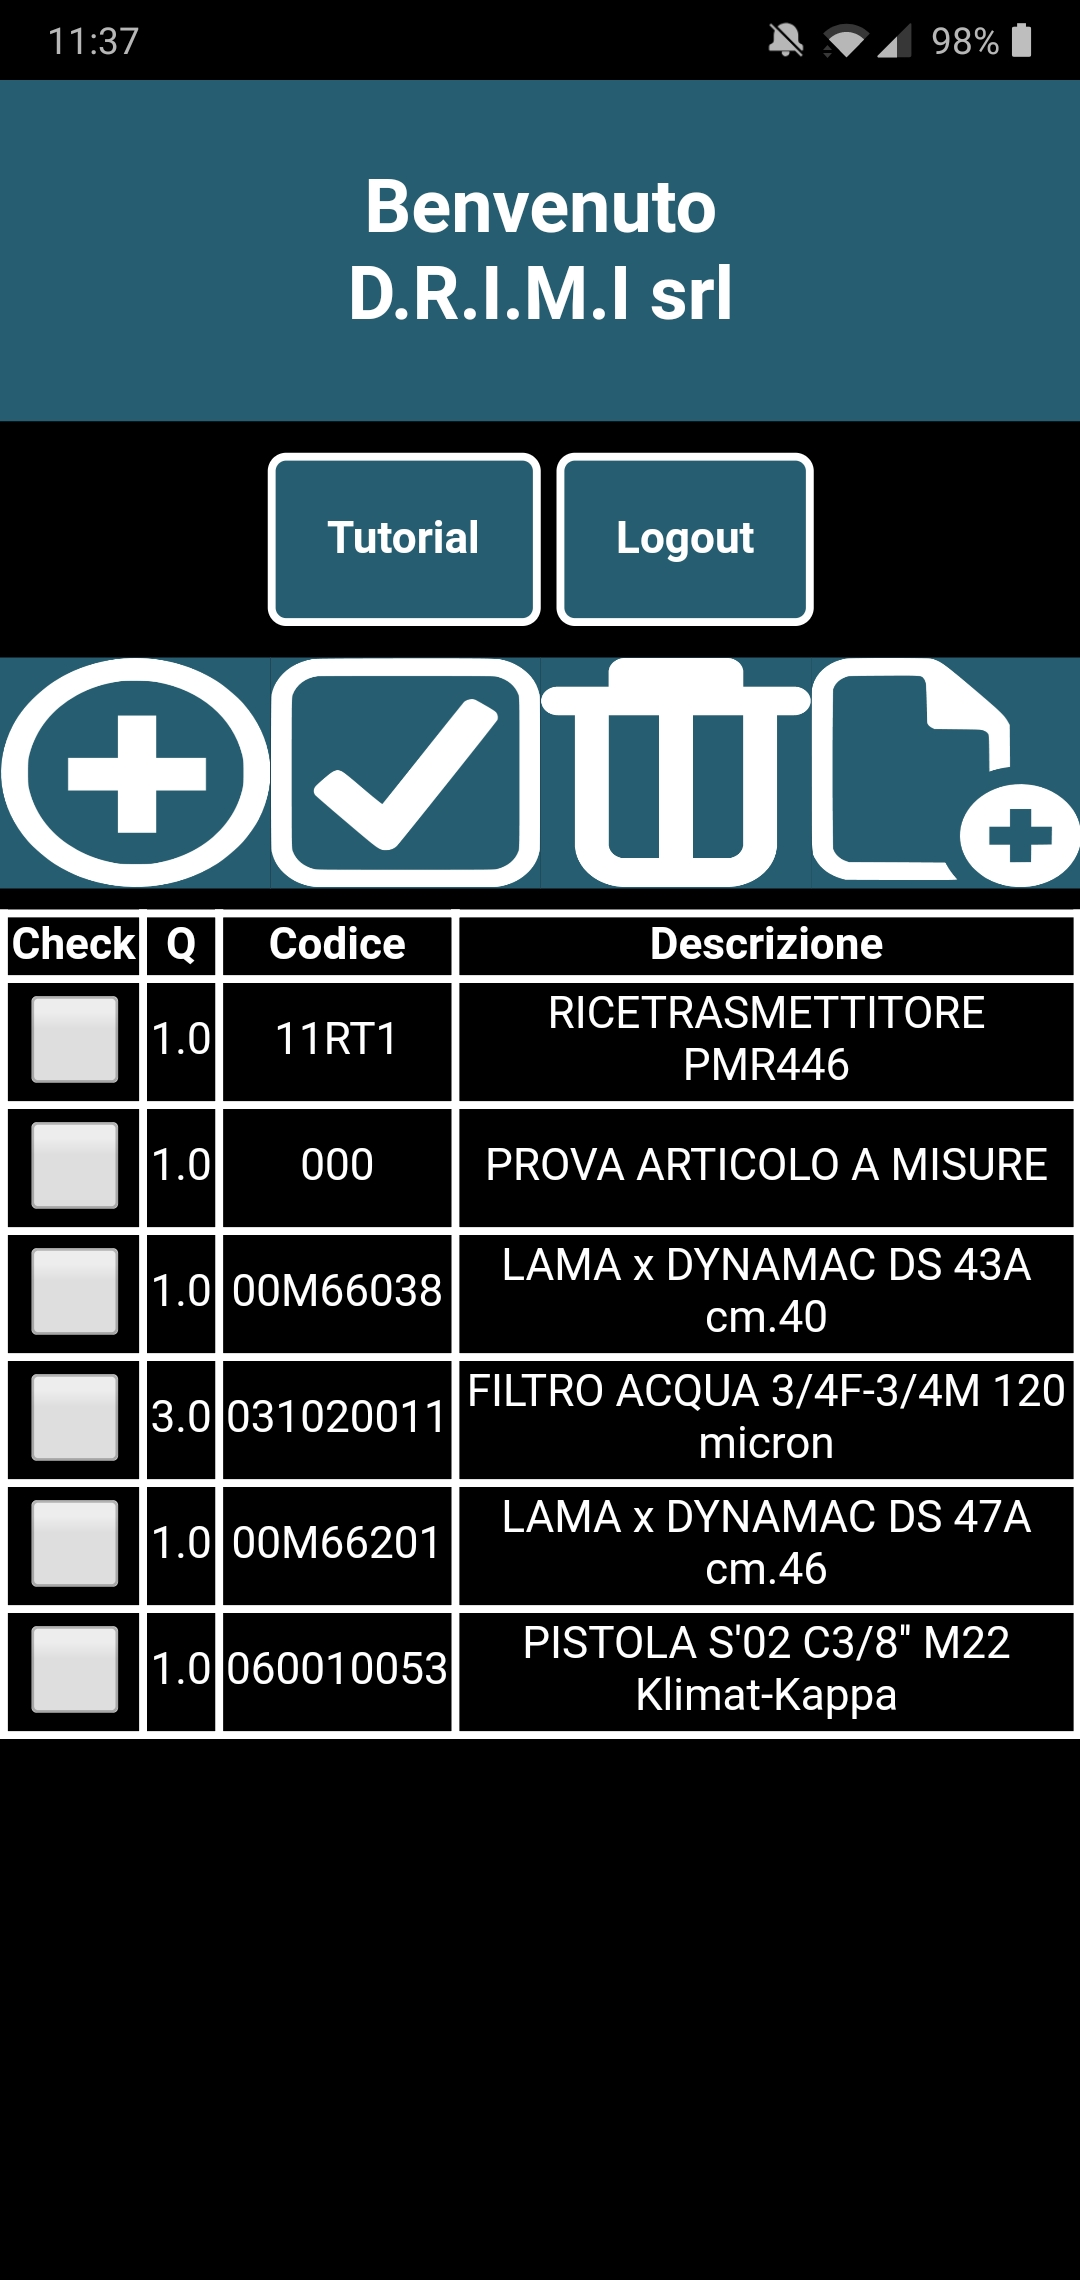
\includegraphics[width=0.4\columnwidth]{interfaccia/home} 
    \caption{\textit{Home page}}
\end{figure}

La \textit{home page} racchiude tutte le funzionalità di \textit{moviORDER}. A partire dall'alto e proseguendo verso il basso, l'interfaccia presenta le seguenti parti:
\begin{itemize}
	\item messaggio di benvenuto per l'utente autenticato: questo messaggio visualizza la ragione sociale dell'utente;
	\item pulsante \textit{tutorial}: premendo su questo pulsante è possibile visualizzare il \textit{tutorial} di \textit{moviORDER};
	\item pulsante \textit{logout}: premendo su questo pulsante è possibile effettuare il logout da \textit{moviORDER};
	\item pulsante di aggiunta articolo: premendo su questo pulsante è possibile accedere al \textit{modal} per l'aggiunta di un articolo in carrello; 
	\item pulsante di selezione/deselezione multipla di articoli: premendo su questo pulsante è possibile selezionare/deselezionare tutti gli articoli in carrello;
	\item pulsante di eliminazione articoli: premendo su questo pulsante è possibile rimuovere gli articoli selezionati dal carrello;
	\item pulsante di invio ordine: premendo su questo pulsante è possibile accedere al \textit{modal} di invio ordine;
	\item carrello: ogni articolo in carrello presenta:
	\begin{itemize}
		\item una check-box per la selezione/deselezione dell'articolo;
		\item un'indicazione sulla quantità di pezzi ordinati;
		\item il codice dell'articolo;
		\item una breve descrizione dell'articolo.
	\end{itemize}
\end{itemize}

\subsection{Modal di aggiunta articolo}

\begin{figure}[!h] 
    \centering 
    	\subfloat{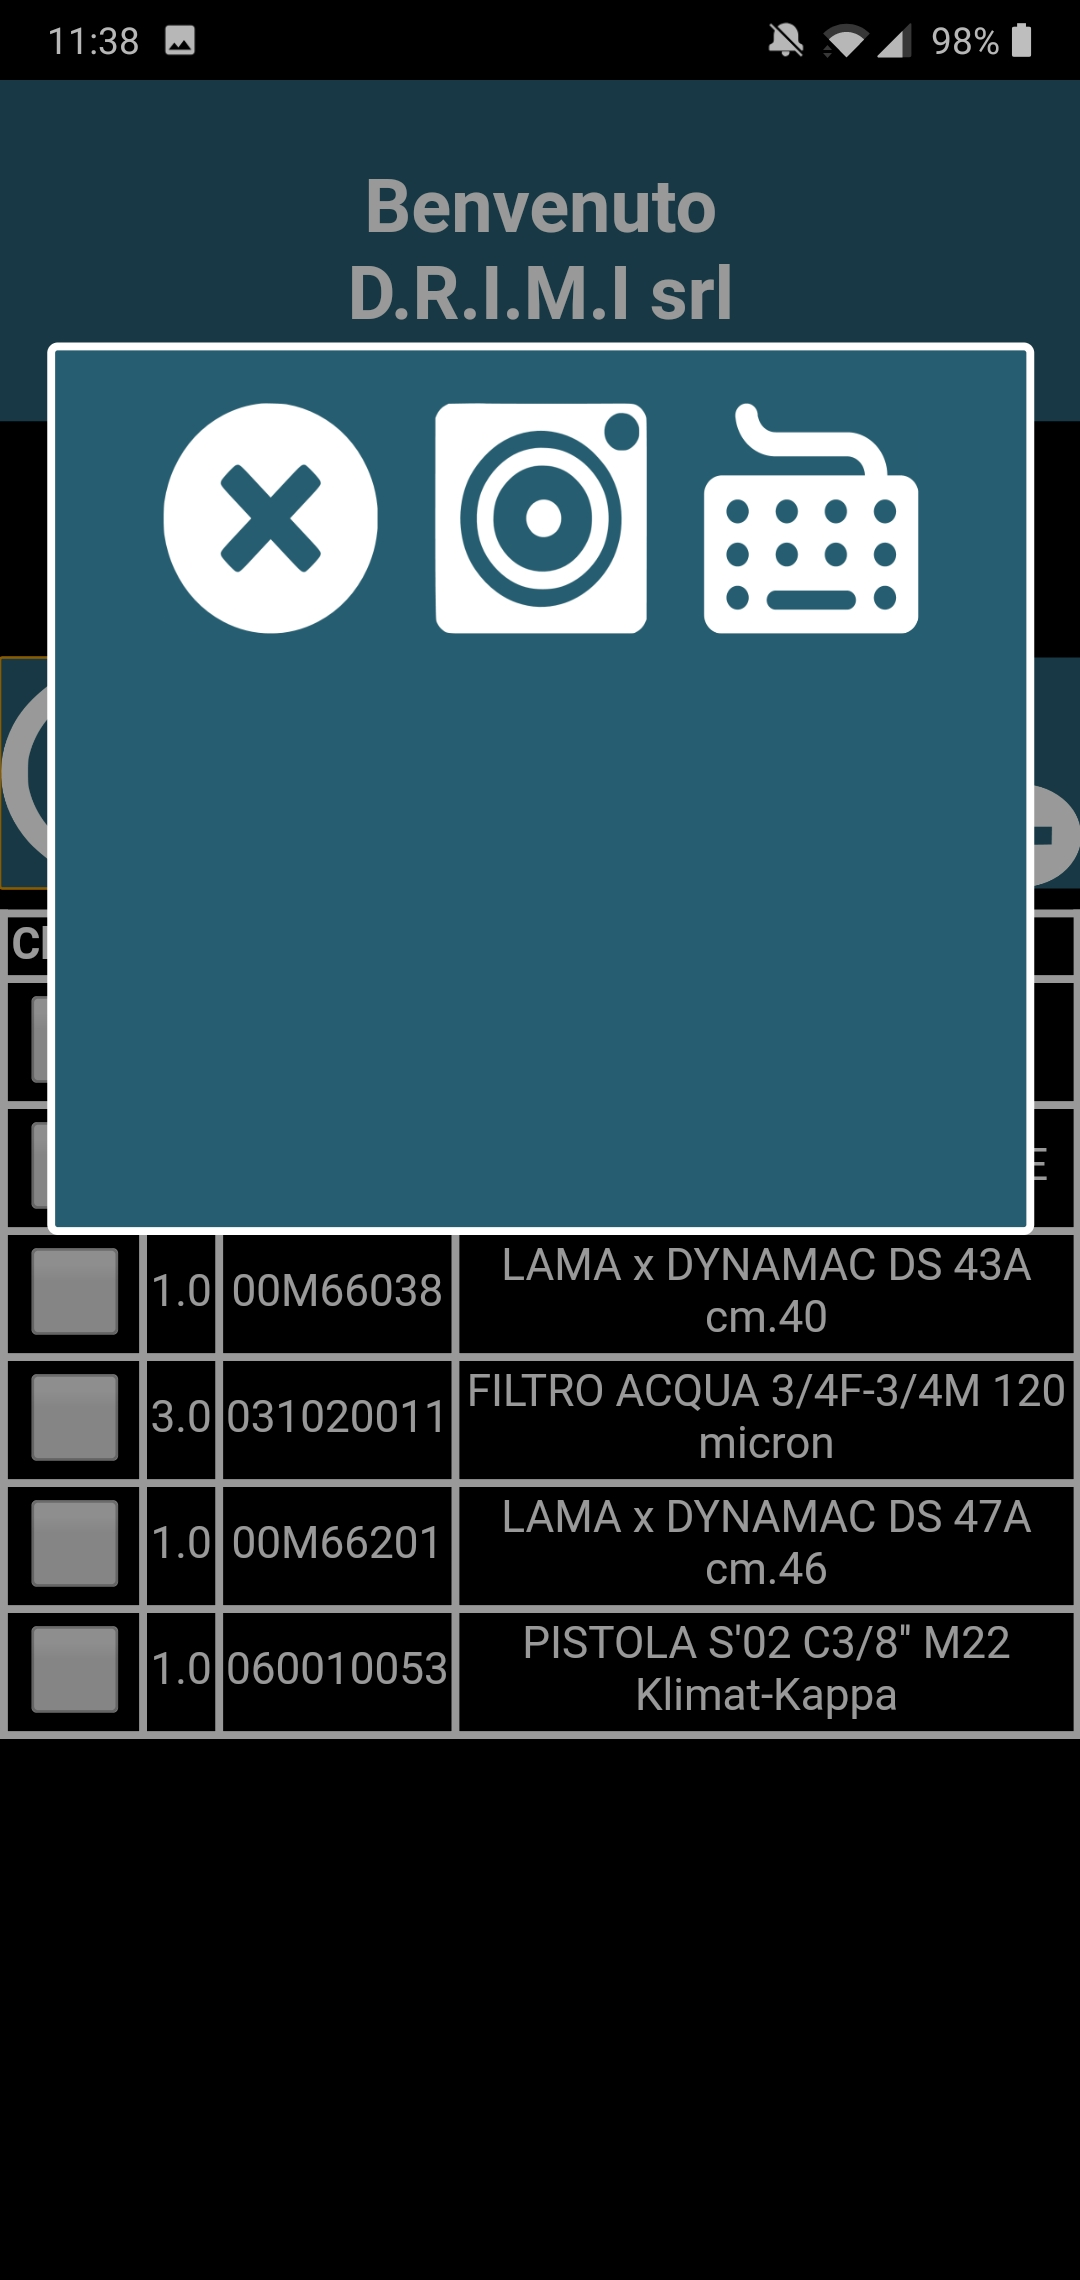
\includegraphics[width=0.33\columnwidth]{interfaccia/modalAggiunta}}
    	\subfloat{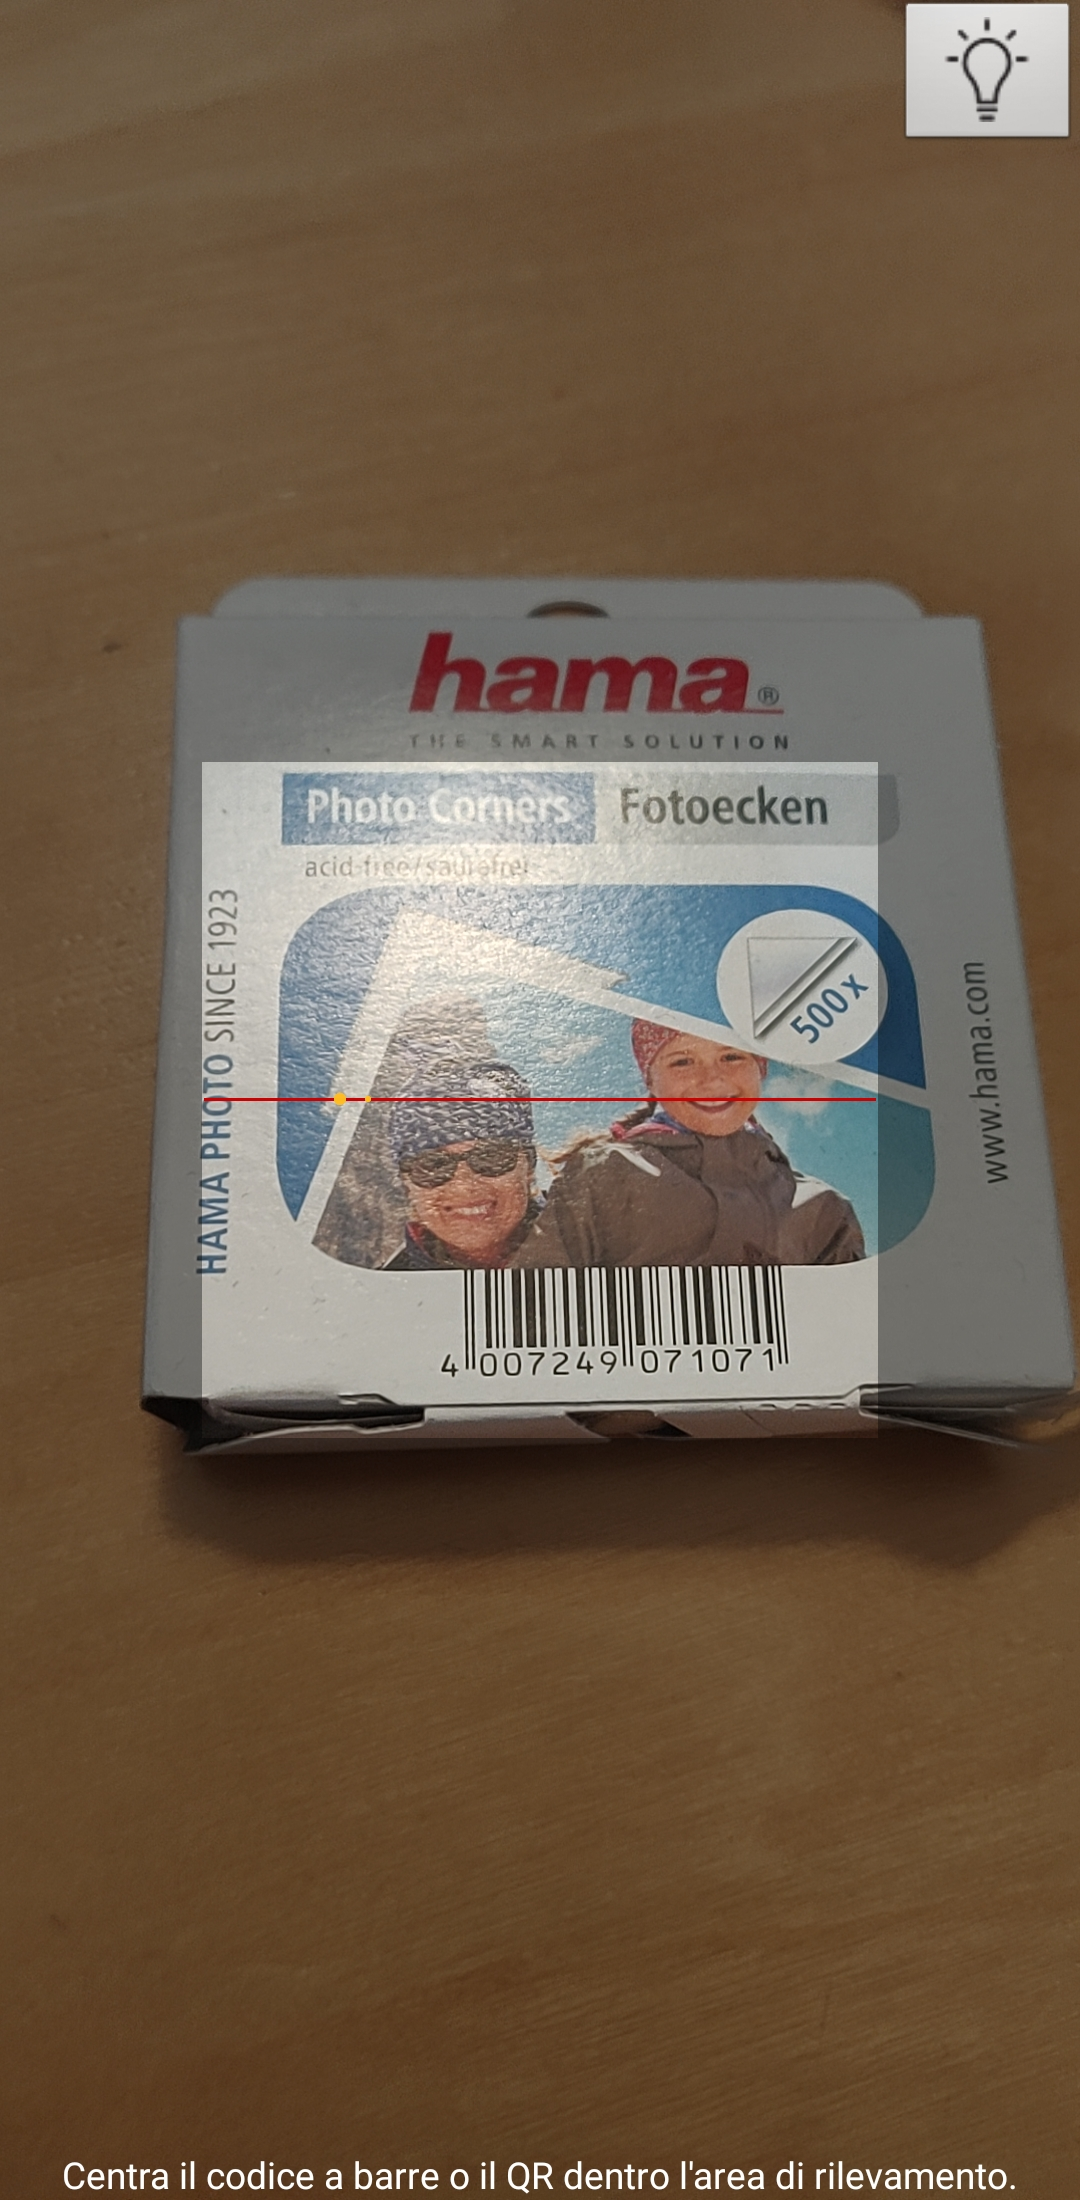
\includegraphics[width=0.33\columnwidth]{interfaccia/scansione}} 
    	\subfloat{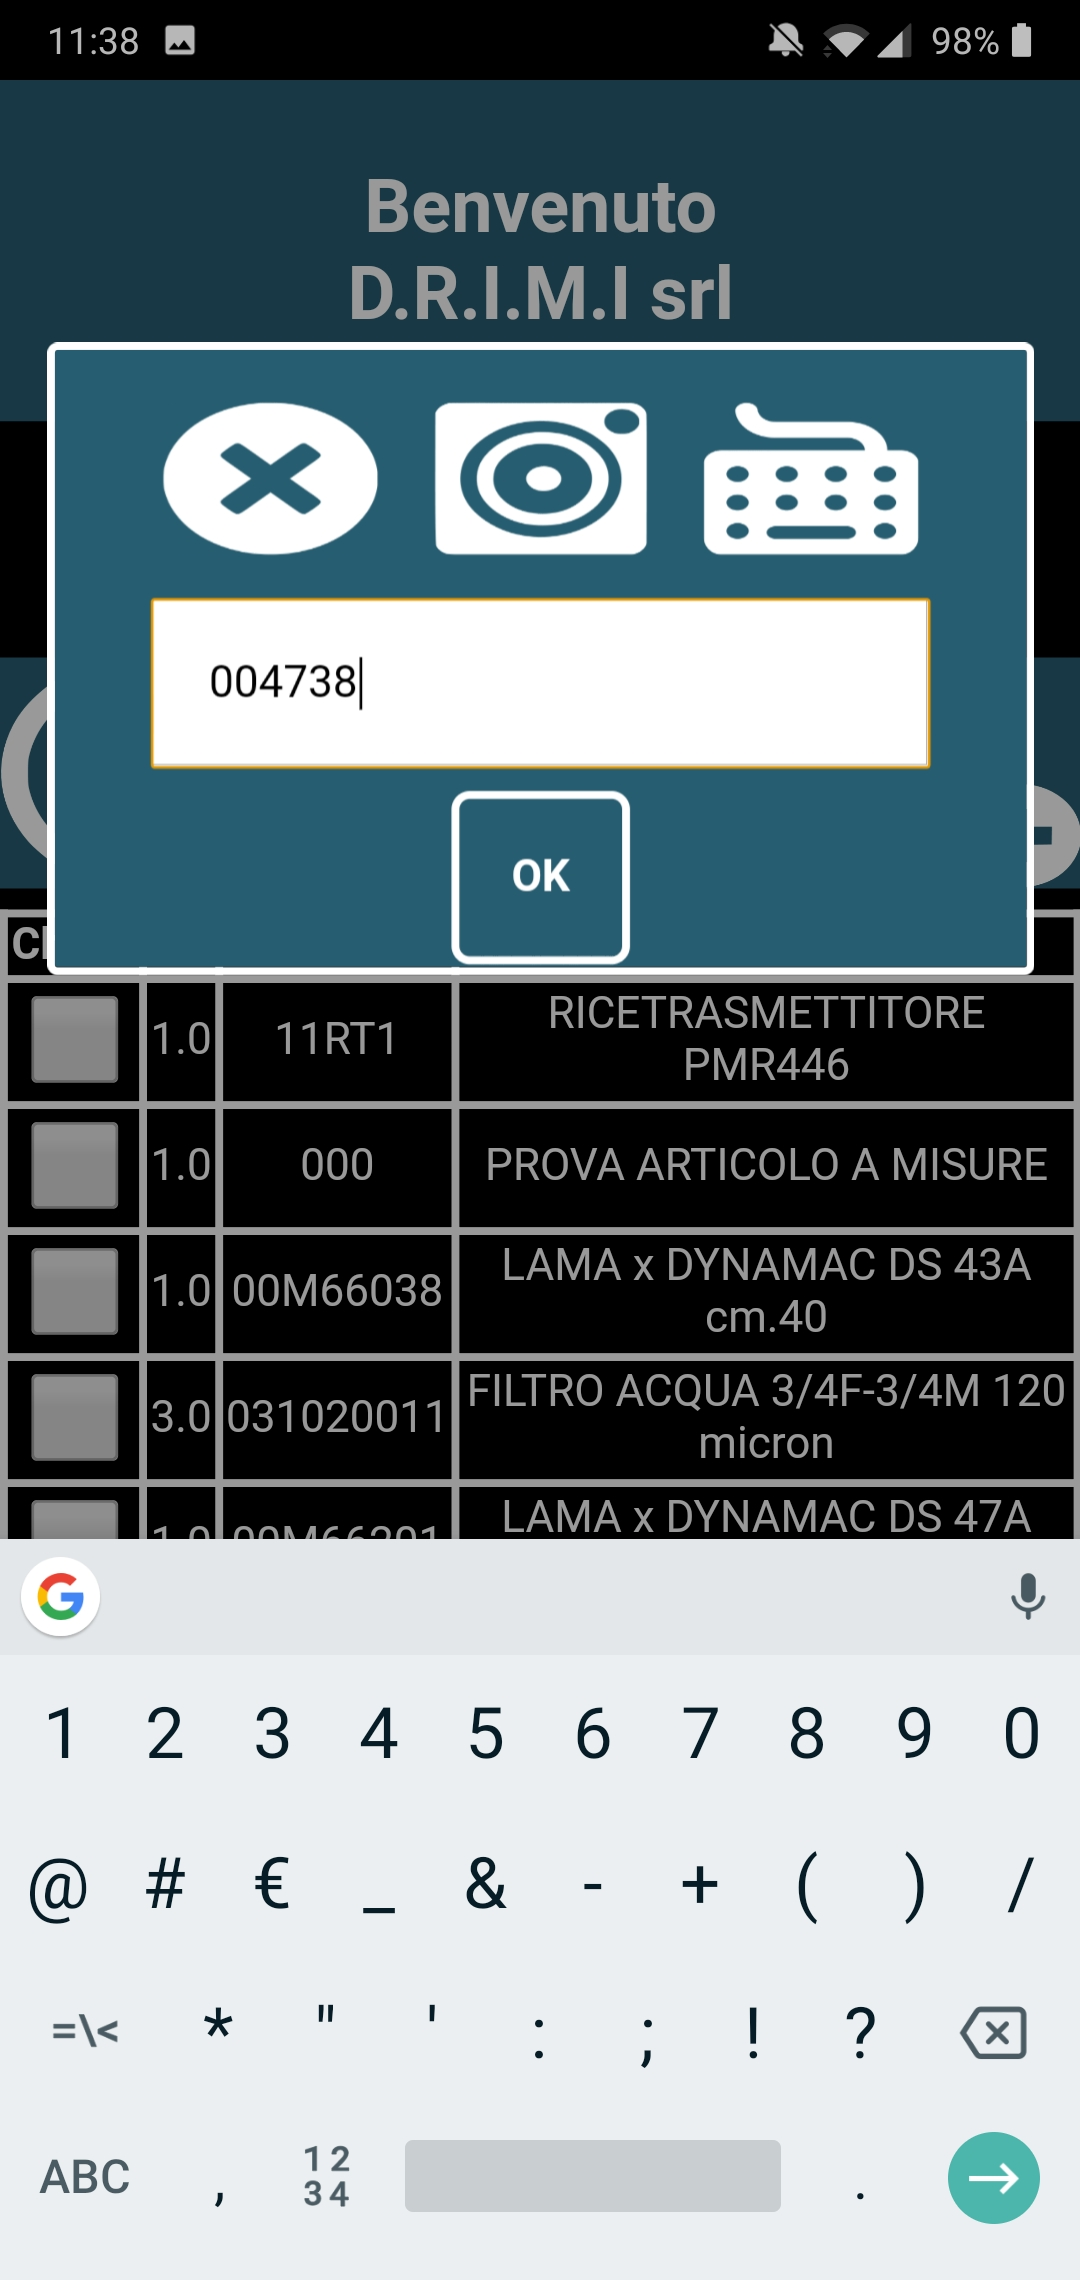
\includegraphics[width=0.33\columnwidth]{interfaccia/manuale}} 
    \caption{\textit{Modal} di aggiunta articolo e modalità di aggiunta (scansione o inserimento manuale)}
\end{figure}

Il \textit{modal} di aggiunta articolo permette di decidere la modalità di inserimento dell'articolo in carrello. Il \textit{modal} presenta i seguenti pulsanti:
\begin{itemize}
	\item annullamento aggiunta: premendo su questo pulsante è possibile tornare alla \textit{home page} di \textit{moviORDER};
	\item scansione codice a barre: premendo su questo pulsante è possibile aggiungere un nuovo articolo scansionando il codice a barre dello stesso. Per la scansione del codice a barre viene aperta la fotocamera del dispositivo;
	\item inserimento manuale: premendo su questo pulsante è possibile aggiungere un nuovo articolo inserendo manualmente il codice dello stesso.
\end{itemize}
Se la scansione del codice a barre o l'inserimento del codice articolo vanno a buon fine, viene aperta la pagina per l'aggiunta dell'articolo corrispondente.

\subsection{Pagina di aggiunta articolo}

\begin{figure}[!h] 
    \centering 
    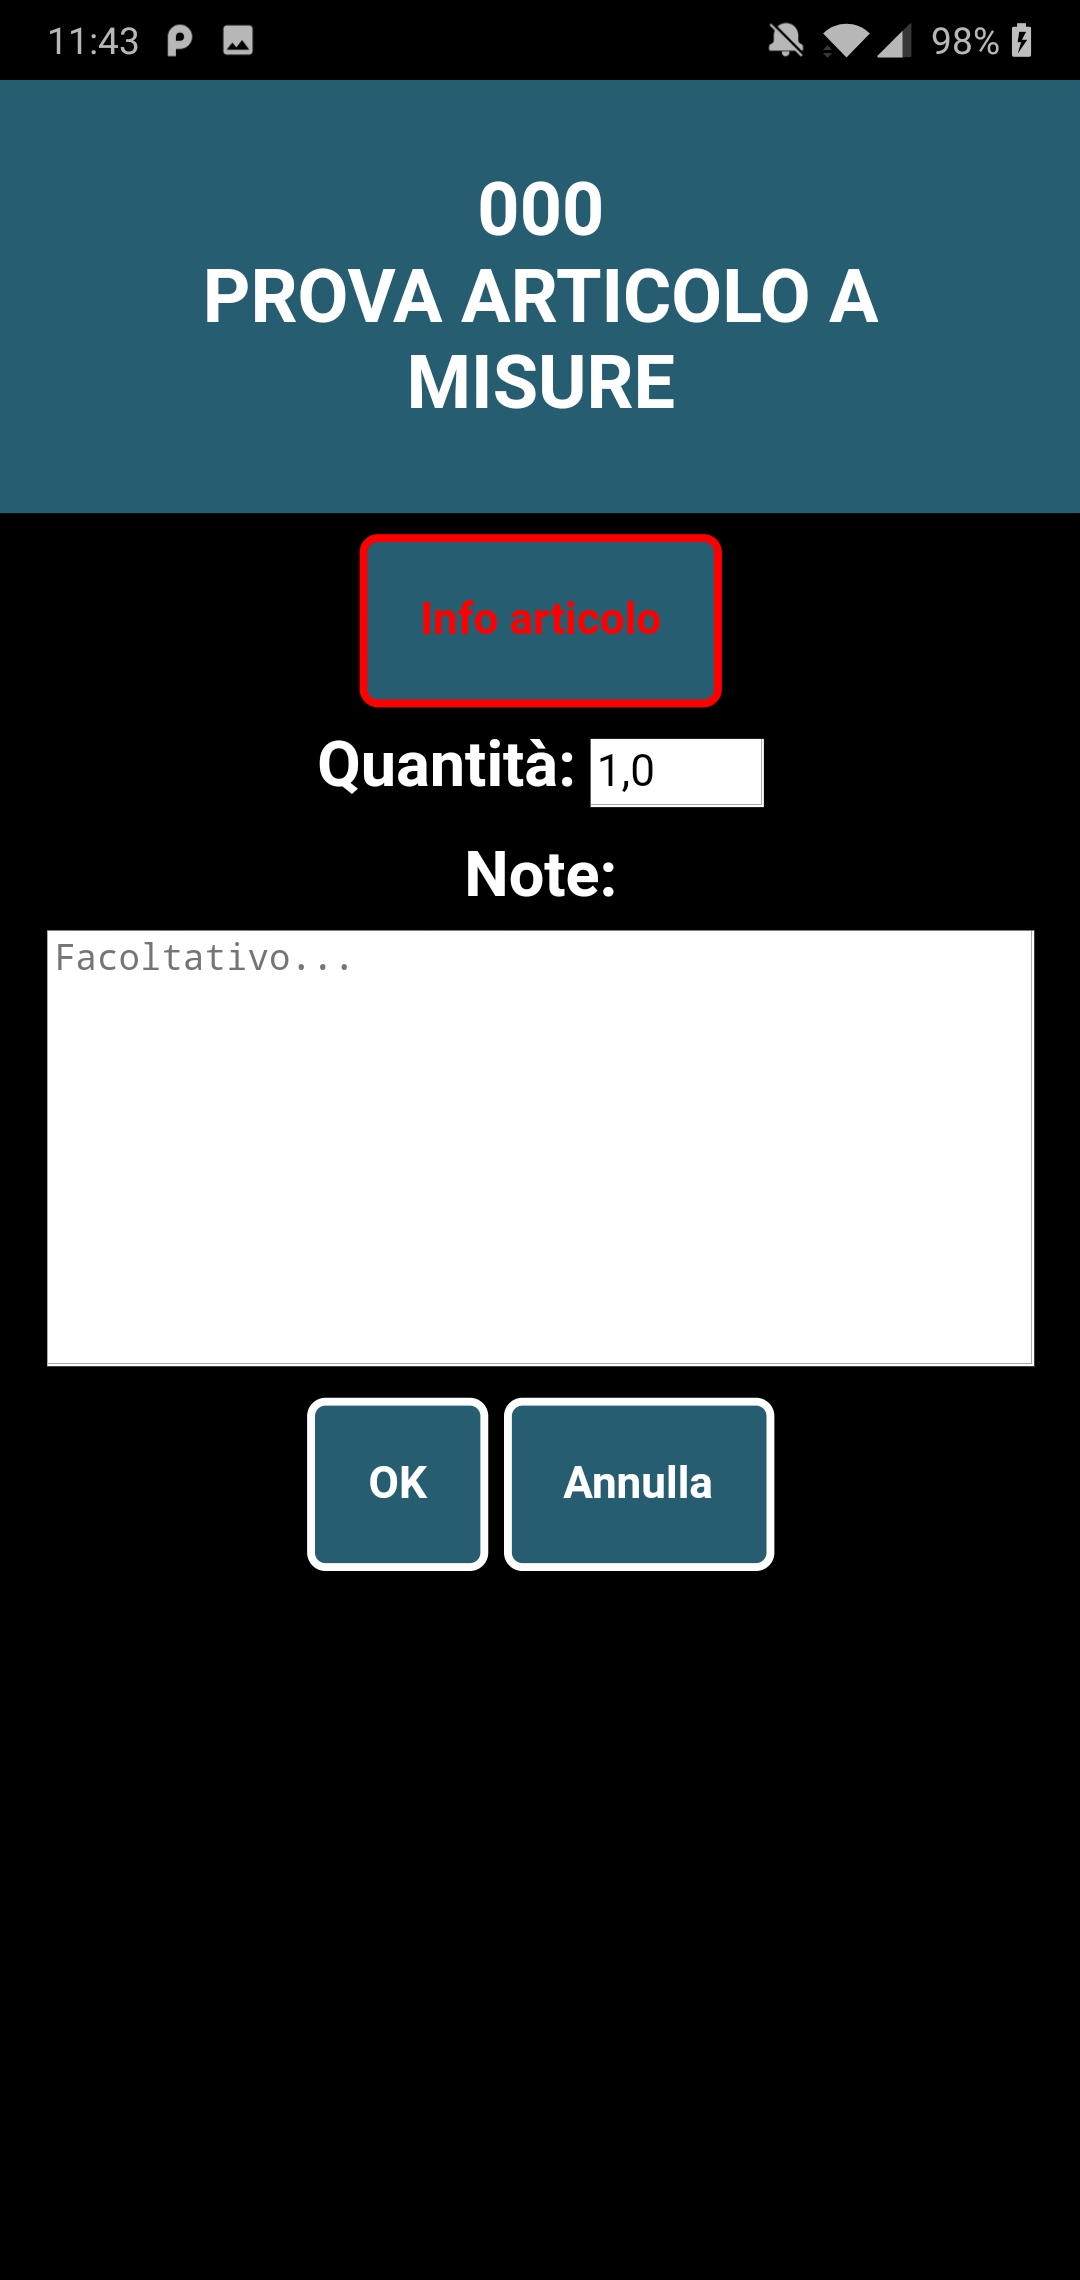
\includegraphics[width=0.4\columnwidth]{interfaccia/aggiunta} 
    \caption{Pagina di aggiunta articolo}
\end{figure}

La pagina di aggiunta articolo permette di aggiungere un nuovo articolo al carrello e presenta le seguenti parti:
\begin{itemize}
	\item codice e nome articolo: in base al codice precedentemente scansionato o inserito, vengono visualizzate le informazioni relative al codice articolo e al nome dell'articolo;
	\item pulsante di visualizzazione informazioni dell'articolo: premendo questo pulsante è possibile visualizzare le informazioni dell'articolo che si sta aggiungendo al carrello. Se il pulsante presenta bordo rosso significa che per l'articolo non sono presenti informazioni. Questo permette all'utente di evitare di pressare inutilmente sul pulsante;
	\item \textit{text-box} per l'inserimento della quantità: tramite questa \textit{text-box} è possibile inserire la quantità da ordinare per l'articolo che si sta aggiungendo al carrello;
	\item \textit{text-area} per l'inserimento delle note: tramite questa \textit{text-area} è possibile inserire delle note facoltative per l'articolo che si sta aggiungendo al carrello;
	\item pulsante di conferma: tramite questo pulsante è possibile confermare l'aggiunta dell'articolo in carrello;
	\item pulsante di annullamento: tramite questo pulsante è possibile annullare l'aggiunta dell'articolo in carrello e tornare alla \textit{home page} di \textit{moviORDER}.
\end{itemize}

\subsection{Pagina di modifica articolo}

Dalla \textit{home page} di \textit{moviORDER}, premendo su un qualsiasi articolo in carrello, è possibile modificare i dati d'ordine di tale articolo. Alla pressione dell'articolo viene aperta la pagina di modifica articolo. Questa pagina è identica alla pagina di aggiunta articolo ma contiene i dati inseriti nel momento in cui si è aggiunto l'articolo in carrello. È possibile modificare tali dati eseguendo le stesse interazioni previste per la pagina di aggiunta articolo.

\subsection{Modal di invio ordine}

\begin{figure}[!h] 
    \centering 
    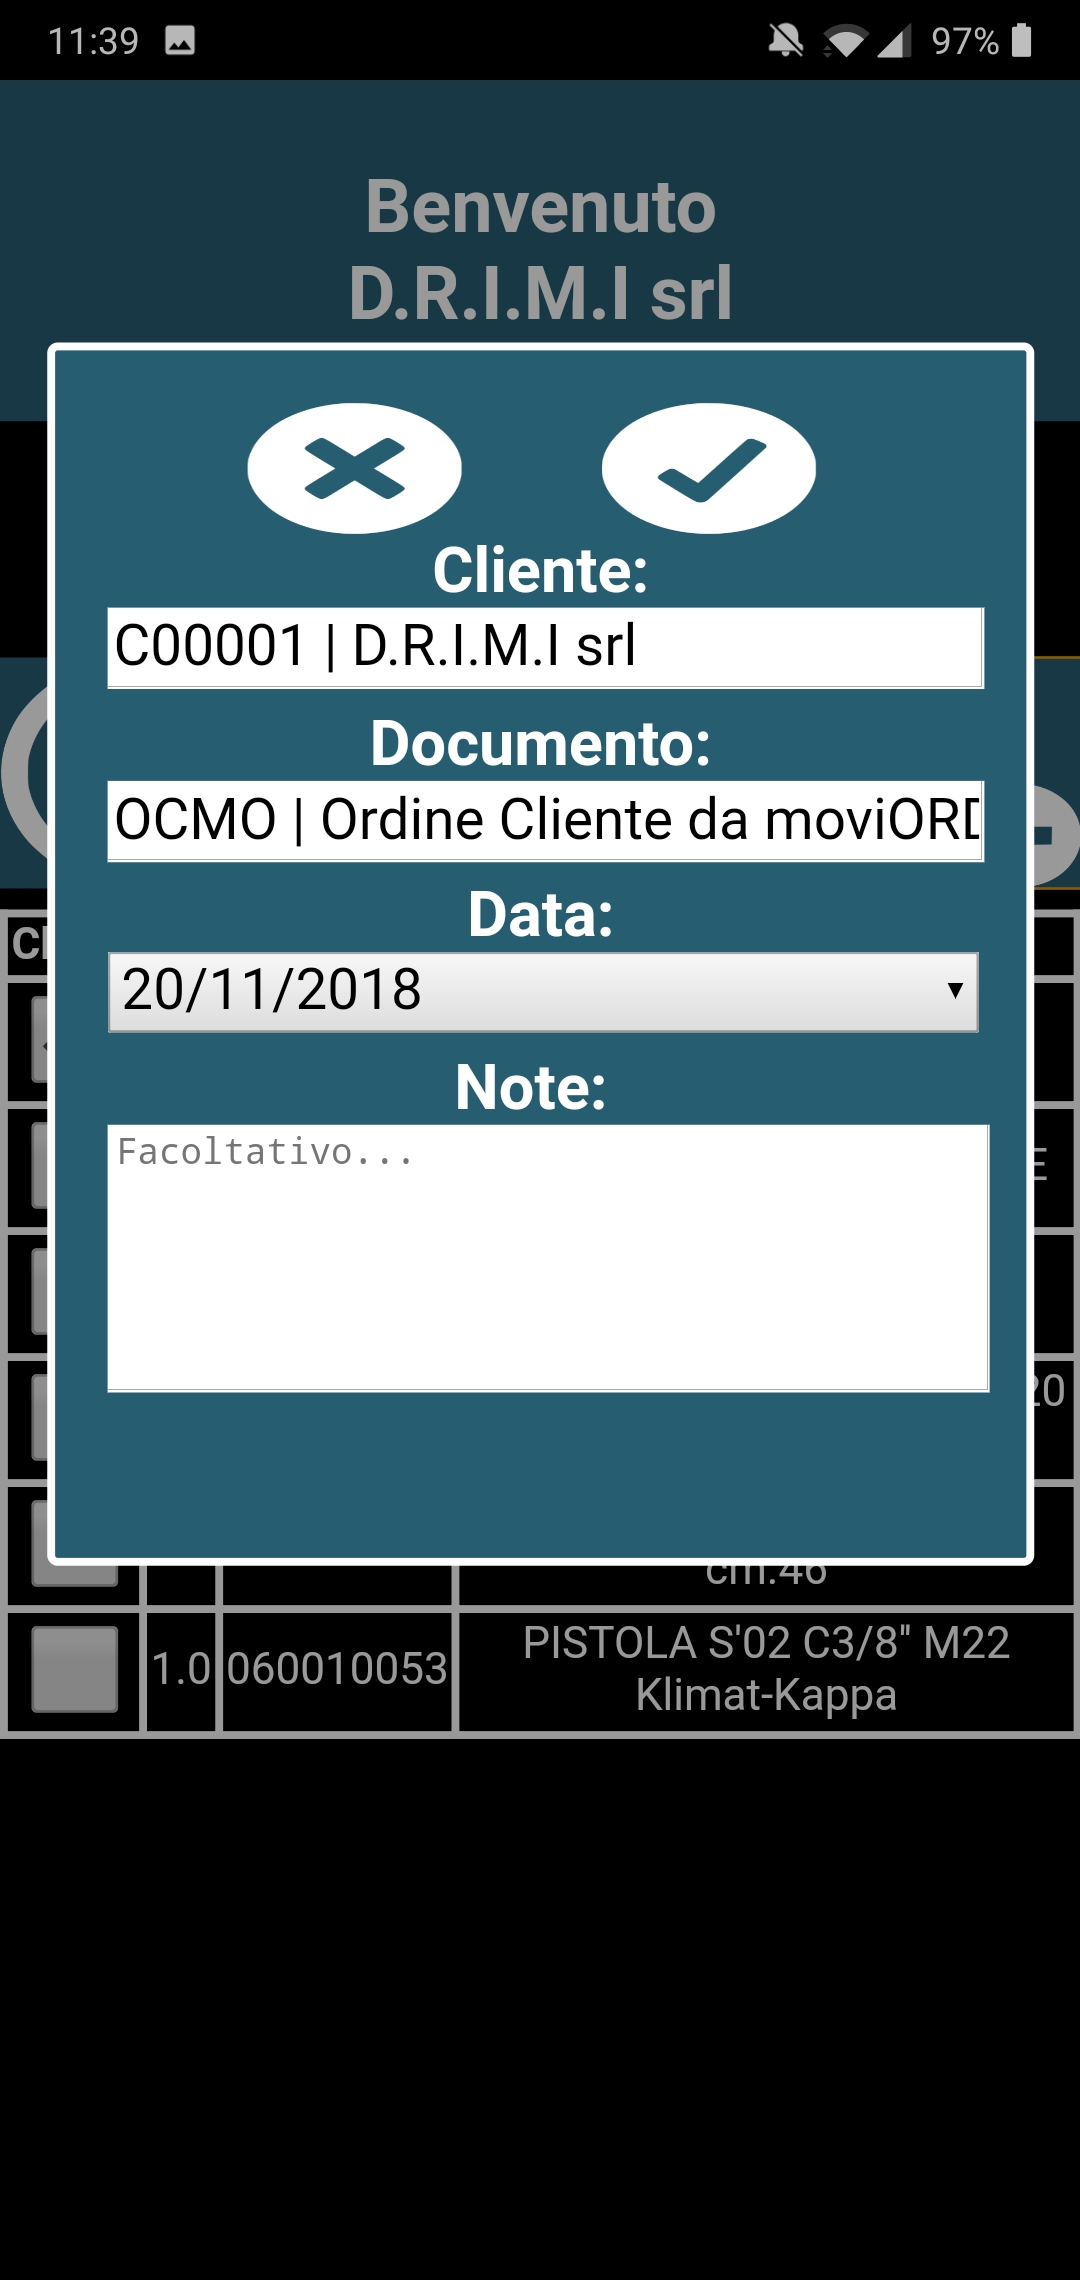
\includegraphics[width=0.4\columnwidth]{interfaccia/modalInvio} 
    \caption{\textit{Modal} di invio ordine}
\end{figure}

Il \textit{modal} di invio ordine permette di inviare un ordine alla propria azienda. Tale ordine contiene tutti gli articoli precedentemente selezionati dal carrello. Il \textit{modal} presenta le seguenti parti:
\begin{itemize}
	\item pulsante di annullamento: premendo questo pulsante è possibile annullare l'invio dell'ordine e tornare alla \textit{home page} di \textit{moviORDER};
	\item pulsante di conferma: premendo su questo pulsante è possibile confermare l'invio dell'ordine;
	\item informazioni sul cliente: \textit{text-box} contenente il codice e la ragione sociale del cliente che sta effettuando l'ordine;
	\item informazioni sul documento: \textit{text-box} contenente il codice e la descrizione del documento che deve essere generato una volta inviato l'ordine;
	\item \textit{select} per l'inserimento della data: questa \textit{select} permette l'inserimento della data d'ordine. Di default viene proposta la data corrente;
	\item \textit{text-area} per l'inserimento delle note: questa \textit{text-area} permette di inserire delle note facoltative per l'ordine che si sta inviando.
\end{itemize}

\begin{figure}[!h] 
    \centering 
    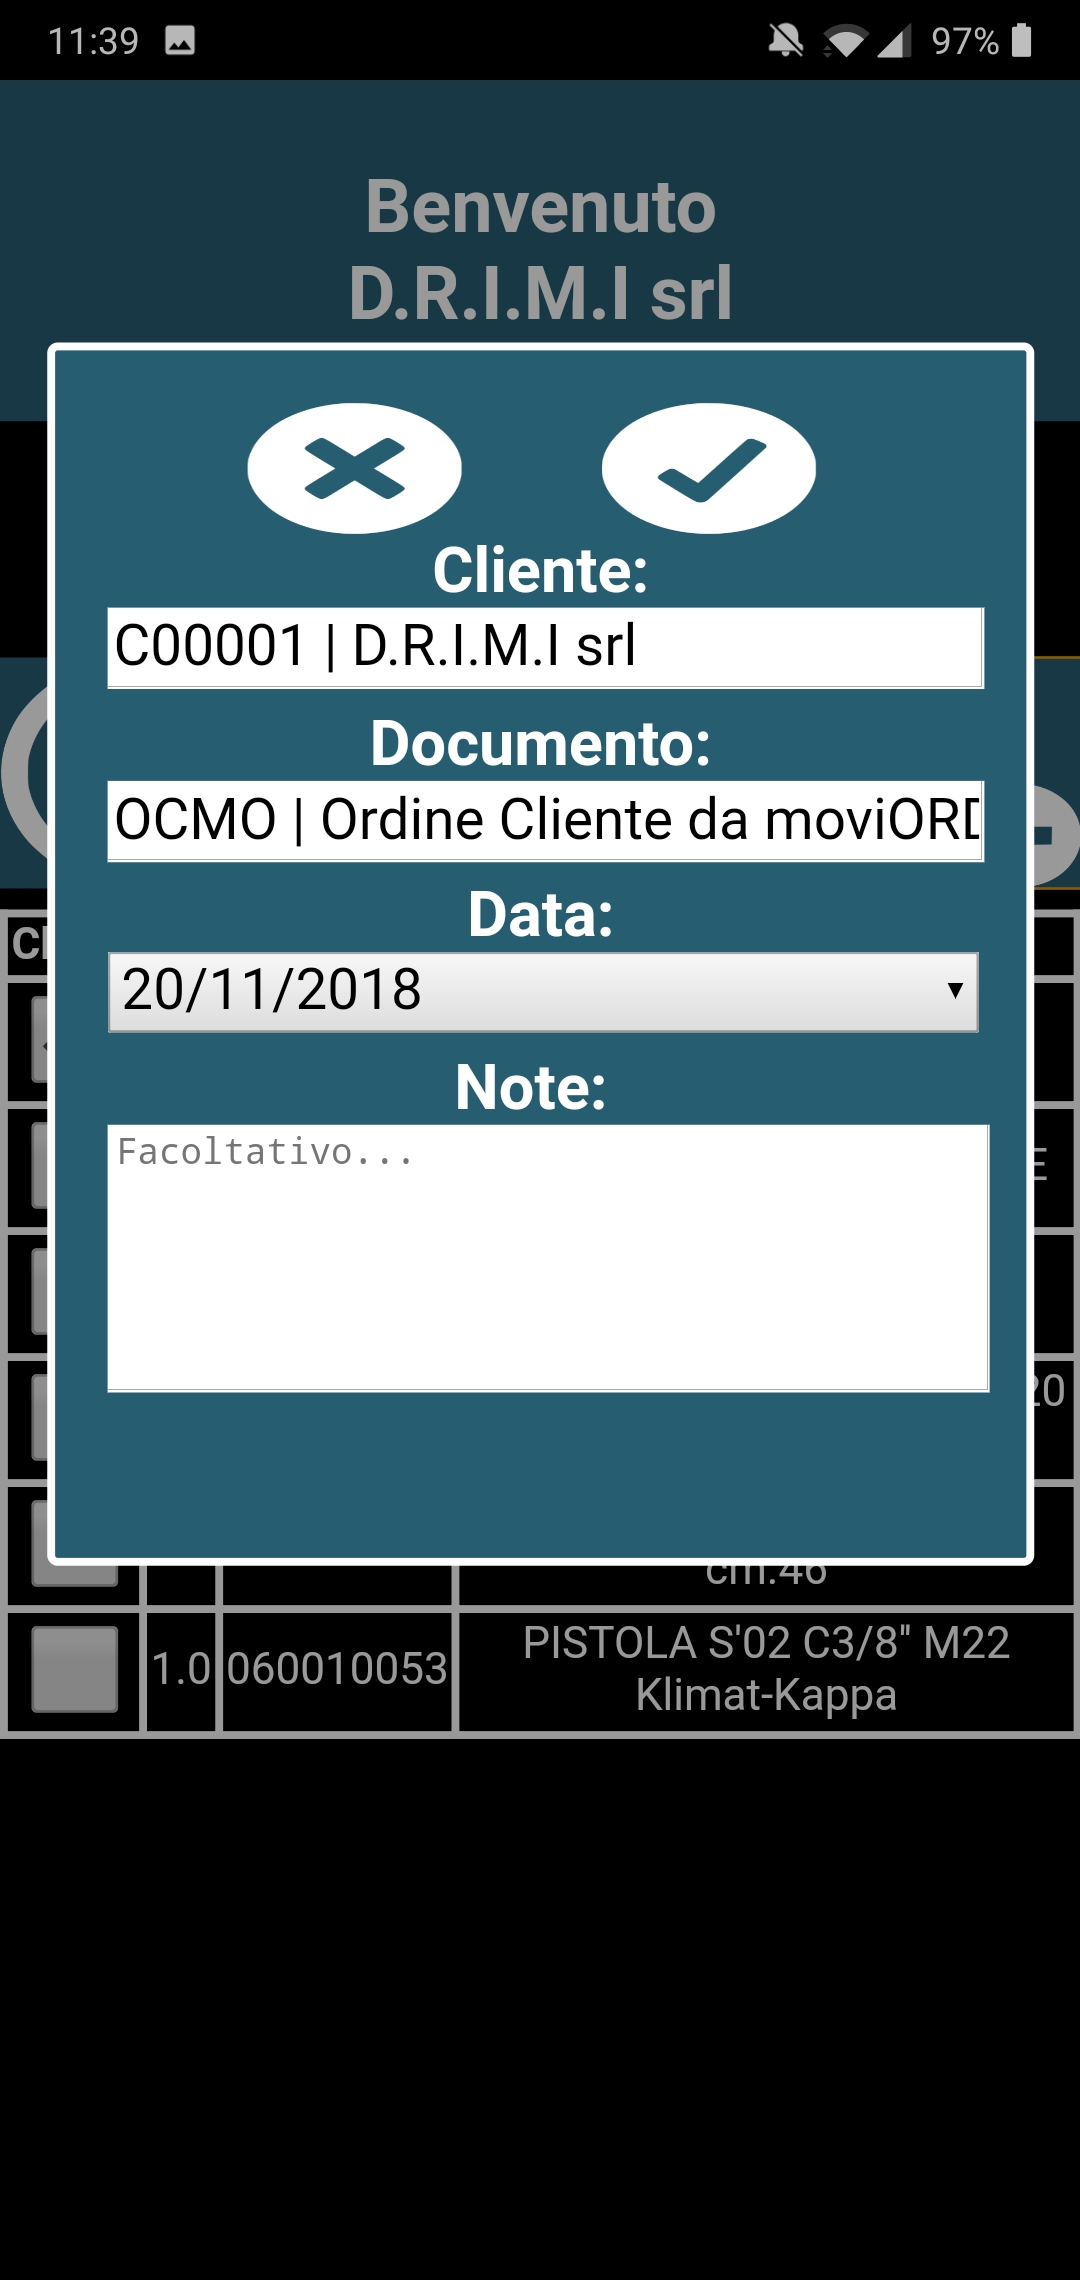
\includegraphics[width=0.4\columnwidth]{interfaccia/modalInvio} 
    \caption{\textit{Modal} di invio ordine}
\end{figure}

\subsection{Considerazioni sullo sviluppo}

L'applicazione \textit{moviORDER} è stata realizzata tramite un framework cross-platform e quindi tramite la realizzazione di un'applicazione web. Per rendere l'applicazione usabile su tutti gli smartphone è stato necessario progettare l'interfaccia dell'applicazione con un approccio \glossaryItem{mobile first} e quindi cercando di realizzare un'interfaccia grafica che fosse più responsive possibile. Per raggiungere questo obiettivo ogni pagina di \textit{moviORDER} presenta un layout elastico che utilizza unità di misura relative (\textit{em} e \textit{\%}) le quali dipendono dalle preferenze dell'utente. Grazie a questo layout, le pagine si adattano correttamente ad ogni dimensione di schermo. Viene di seguito fornito, a scopo illustrativo, un esempio di codice \textit{css} che utilizza unità di misura relative per la rappresentazione degli elementi dell'interfaccia.

\begin{figure}[!h] 
    \centering 
    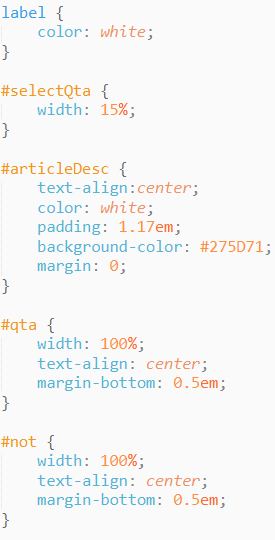
\includegraphics[width=0.5\columnwidth]{codice/css} 
    \caption{Codice \textit{css} che utilizza unità di misura relative}
\end{figure}